%\documentclass[prb,11pt]{revtex4}
\documentclass[twocolumn]{revtex4}

\usepackage{amsfonts, amsmath, amssymb, mathrsfs}
\usepackage{verbatim}
\usepackage{url}
\usepackage[pdftex]{graphicx}           % Standard graphics package
\usepackage{epstopdf}

\renewcommand{\thefootnote}{\fnsymbol{footnote}}
\def\be{\begin{eqnarray} &&} 
\def\nonu{\nonumber \\ &&} 
\def\ee{\end{eqnarray}} 
\def\nonu{\nonumber \\ &&} 
\date{\today}
%\maketitle

\begin{document}

\title{Exposing Novel Quark and Gluon Effects in Nuclei}

\author{I.~Clo\"et}
\affiliation{Physics Division, Argonne National Laboratory, Argonne, IL 60439, USA}

\author{R.~Dupr\'{e}}
\affiliation{Institut de Physique Nucl\'eaire, CNRS-IN2P3, Univ. Paris-Sud, Universit\'e Paris-Saclay, 91406 Orsay Cedex, France}

\author{S.~Riordan}
\thanks{Corresponding author}
\email{sriordan@anl.gov}
\affiliation{Physics Division, Argonne National Laboratory, Argonne, IL 60439, USA}

\author{W.~Cosyn}
\affiliation{Ghent University, Gent, Belgium}

%\author{W.~Armstrong}
%\affiliation{Argonne National Laboratory, Lemont, IL 60439, USA}

\author{J.~Arrington}
\affiliation{Physics Division, Argonne National Laboratory, Argonne, IL 60439, USA}

\author{N.~Fomin}
\affiliation{Univesity of Tennessee, Knoxville, TN 37996, USA}

\author{A.~Freese}
\affiliation{Physics Division, Argonne National Laboratory, Argonne, IL 60439, USA}

\author{D.~Gaskell, C.~E.~Keppel}
\affiliation{Thomas Jefferson National Accelerator Facility, Newport News, VA 23606, USA}

\author{G.~Miller}
\affiliation{University of Washington, Seattle, WA 98195, USA}

\author{E.~Pace}
\affiliation{University of Florence, Florence, Italy}

\author{S.~Platchkov}
\affiliation{Saclay University, Paris, France}

\author{P.~E.~Reimer}
\affiliation{Physics Division, Argonne National Laboratory, Argonne, IL 60439, USA}

\author{S.~Scopetta}
\affiliation{Universit\`{a} di Perugia, Sezione di Perugia, Italy}
\affiliation{INFN, Sezione di Perugia, Italy}


\author{A.~Thomas}
\affiliation{University of Adelaide, SA 5005, Australia}

\author{P.~Zurita}
\affiliation{Physics Department, Brookhaven National Laboratory, Upton, NY 11973, USA}

\keywords{EMC effect; medium modification; nuclear modification; tagged scattering; deep inelastic scattering; nuclear generalized parton distributions; gluon distributions; parton distributions; short}

\begin{abstract}
    The modification of protons and neutrons in the nuclear medium presents a major challenge for modern nuclear physics.  After several decades of the first observation of modification through the EMC effect, there remain a number of important open questions to be addressed, including the flavor, spin, and momentum dependence of modification.  In this paper we briefly review the state of the field, explore a range of new opportunities to better understand modification, and present a set of key questions and programs to address them.
\end{abstract}

\maketitle
\section{Introduction}


Understanding the emergence of nuclei within QCD is a key challenge for modern science.  Since the advent of QCD, the role of quarks and gluons in nuclei relative to their counterparts in free protons and neutrons is unclear.  Traditional nuclear physics approaches the problem as comprised of many body hadronic states and has had significant success in describing the properties of nuclei across the chart of nuclides. However, because QCD is the fundamental theory of the strong interaction, it is unlikely that these hadron-level approaches can remain valid, or contain the correct degrees of freedom, for all processes at all energy scales. Clearly identifying these scales and processes is key to exposing the role of quarks and gluons in nuclei and thereby developing an understanding of how nuclei emerge within QCD.

In order to gain a detailed picture of the partonic structure of nuclei, a broad program must be developed on several fronts.  This includes novel measurements of nuclear structure with high energy leptonic probes, with inclusive, semi-inclusive and exclusive final states, Drell-Yan processes with different incident hadrons, a rigorous development of theoretical frameworks and modeling, and  careful constraint and understanding of systematic effects.

There are several key questions to be answered which are within the reach of the physics community which would broadly expand upon our present knowledge of medium modification.  This includes the nature of the isovector aspects of modification across many nuclei, the dependence on nuclear spin, the relation to the momenta of the bound internal quarks and hadronic constituents, and the full femtoscopic imaging of the nucleus.  Coupled with these studies is the need for a rigorous formalism and a better understanding of the systematic effects such as in hadronization and the nuclear longitudinal structure functions. 

In this paper, we summarize the current experimental and theoretical state of knowledge and put forth a road map and key set of questions for the next era of measurements and calculations.  These new directions in experiment and theory will cover needed information for the latest nuclear parton distribution functions, programs which will study the spin and isospin-dependence of modification, better constrain both valence and sea distributions, and ultimately achieve a more complete tomography of the structure of nuclei.

%\textbf{Notes from board}\\
%Introduction -- broad questions, why nuclei? \\
%Status  - Present, PDFs, SRC, Theory (basically Dave's)\\
%New Directions - IVEMC, SPIN, DY, Nuclear GPDs and light nuclei, Tagged\\
%Systematics - Hadroniztion, analysis of PDF, d/u\\
%Summary/Road Map - new key measurements, calculations, formalism\\

\section{Status of the EMC effect}

One of the best tools available for studying the internal structure of nucleons is the deep inelastic
scattering (DIS) process, where a charged lepton scatters inelastically with a large four-momentum
transfer represented by the Lorentz invariant $Q^2 = -q^2 = q^\mu q_\mu \gg 1-2~\mathrm{GeV}^2$.
The process is characterized by a scaling variable Bjorken-x, $x = Q^2/2M_N \nu$, 
where $M_N$ is the mass of the target hadron and $\nu$ is the energy transfered from the lepton in the laboratory frame,
which is associated with the momentum fraction carried by a struck spin-1/2 partons in the limit of the infinite momentum frame.
To leading order the unpolarized electromagnetic DIS cross section in the laboratory frame can be written~\cite{PhysRevD.98.030001}
\begin{equation}
    \frac{d^2 \sigma}{dx dy} = \frac{4 \pi \alpha^2}{x y Q^2} \left[ (1-y)F_2(x, Q^2) + y^2 x F_1 \right]
\end{equation}
where $y = \nu/E$ where $E$ is the incident lepton energy, $\alpha$ is the fine structure constant and $F_2$
and $F_1$ are structure functions of the proton to be determined.  These structure functions can be reduced
by the Callan-Gross relation $F_2 - 2xF_1 = F_\mathrm{L} \approx 0$ for non-interacting point-like spin-1/2
particles with
\begin{equation}
    F_2(x,Q^2) = x \sum_{q} e_q^2 q(x,Q^2)
\end{equation}
where the sum $q$ is over all quark flavors,  $e_q$ is the electromagnetic chare of the quark, and the
functions $q(x,Q^2)$ are the parton distribution functions (PDFs) which are believed to be universal
and can describe other processes such as Drell-Yan.  Analagous distributions exist for the case of polarized
targets.  A great success of QCD is the prediction of the logarithmic 
evolution of the PDFs with $Q^2$, the so-called DGLAP evolution.  These PDFs can in principle be measured for any bound hadronic state.

The EMC effect~\cite{Aubert:1983xm} is the observation that the PDFs for nuclei are different than
the incoherent sum over the PDFs of the constituent nucleons and marks a clear sign of the modification
of the structure of the nucleons when bound together in a nucleus.
Since the original discovery in 1983, there has been a large
program of measurements at several laboratories, such as CERN, Fermilab, SLAC, DESY, and Jefferson Lab (JLab),
aimed at understanding the properties and probing the origin of the nuclear dependence of inelastic
structure functions (see~\cite{Geesaman:1995yd, Malace:2014uea, Hen:2016kwk} for reviews related to the EMC effect).
Measurements with high energy (of scale 100 GeV) muon beams have provided high-precision data at low to
moderate $x$ ($<0.3$), while more modest energy electron facilities (of scale 10 GeV) have provided
the highest precision at large $x$ ($>0.3$), Fig.~\ref{fig:emc_iron}.  The low-to-moderate $x$
regions show interesting shadowing and anti-shadowing behaviors, while the suppression of the
per-nucleon cross section for $0.3<x<0.7$ is the hallmark of the EMC effect.

The most comprehensive data set with high precision at large $x$ comes from SLAC E139. This experiment
measured the EMC effect for a wide range of nuclei, from $^4$He to Au with good precision up to
$x\approx0.8$.  One of the outcomes of E139 was an investigation of the detailed nuclear dependence of the EMC
Effect. It was found that the nuclear dependence of the EMC effect at large x ($x=0.6$) is consistent
with both a logarithmic $A$ dependence as well as a linear dependence on average nuclear density.

From the measurements made prior to the Jefferson Lab program, one can draw several conclusions about
the global properties of the EMC effect:
\begin{enumerate}
 \item{The shape of the EMC effect (shadowing, anti-shadowing, and EMC regions at small, moderate, and
  large $x$ respectively) is universal and observed in all nuclei.}
 \item{The EMC effect displays little $Q^2$ dependence over the full $x$ range.}
 \item{At large $x$, the EMC effect grows with $A$, while there is little apparent $A$ dependence in the
   anti-shadowing region.}
\end{enumerate}

%%%theory
Since the first observation of the EMC effect, many theoretical models have been proposed and can be subdivided into two categories.  One includes only ``traditional'' nuclear physics effects, using convolution models with binding effects, detailed models of the nucleon momentum distribution, or pion-exchange contributions. The other category invokes more exotic explanations such as re-scaling of quark distributions in the nuclear environment, contributions of six or nine
quark bags, or modification of the internal structure of the nucleons such as ``nucleon swelling'' or suppression of point-like nucleon configurations. Several reviews give an overview of models of the EMC effect~\cite{Geesaman:1995yd, Norton:2003cb, Piller:1999wx, Hen:2013oha, Malace:2014uea}.


\begin{figure}[htb]
  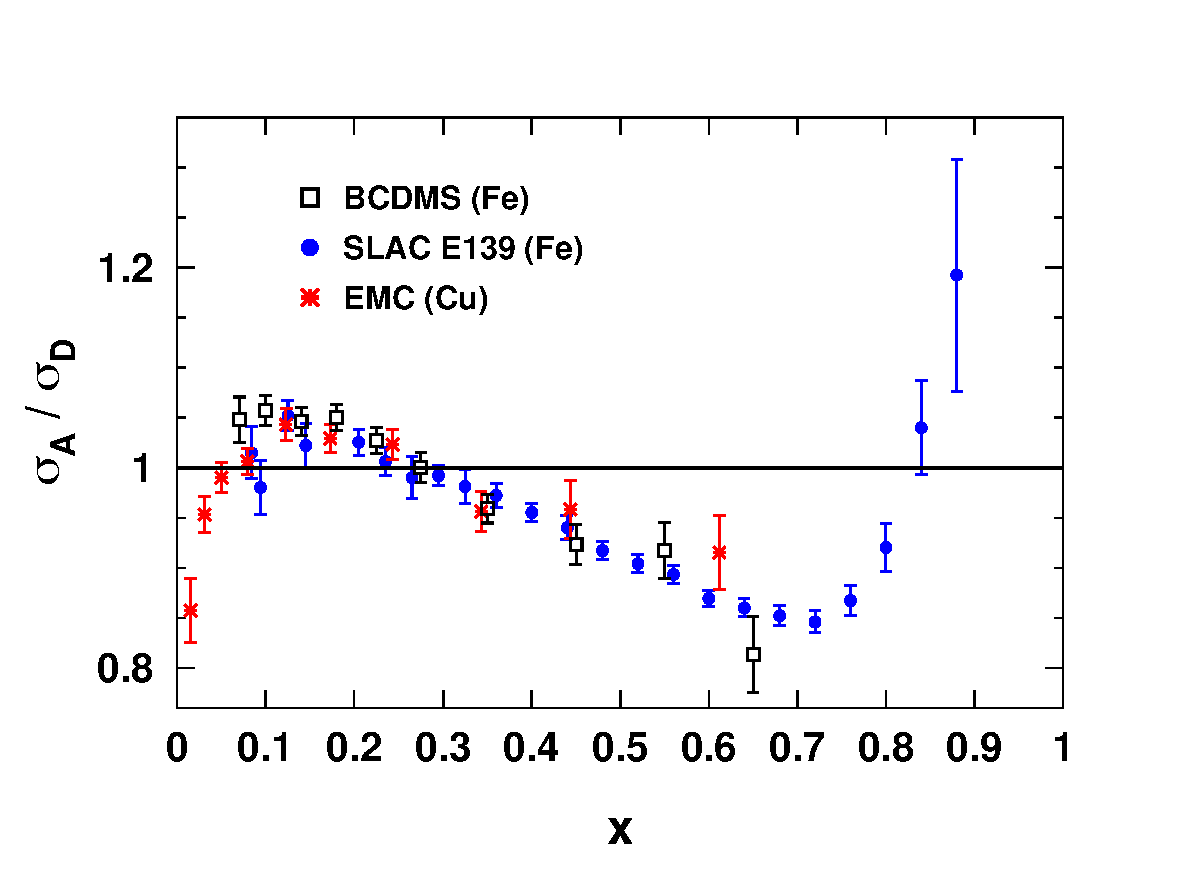
\includegraphics[width=0.5\textwidth]{plots/emc_cu_fe.pdf}
  \caption{EMC effect for iron (BCDMS collaboration~\cite{Benvenuti:1987az} and SLAC E139~\cite{Gomez:1993ri})
    and copper (EMC collaboration~\cite{Ashman:1992kv}).
    Figure from Ref.~\cite{Guzey:2012yk}}
  \label{fig:emc_iron}
\end{figure}

\subsection{EMC effect results from Jefferson Lab and the EMC-SRC correspondance}

The primary goal of Jefferson Lab E03-103 was to augment the results obtained from SLAC E139 by taking
advantage of improved target technologies to provide higher precision data for $^4$He and the first
measurement of the EMC effect from $^3$He at large $x$.  Additional light (Be and C) and heavy (Cu and Au)
targets were also used to provide improved precision at large $x$.

Since the shape of the EMC effect is universal, the E03-103 analysis defined the ``size'' of the EMC
effect as the slope of a line fit between $0.35<x<0.7$.  This definition reduces sensitivity to
normalization uncertainties and results in higher sensitivity to the nuclear dependence.

The slope of the EMC effect for $^3$He, $^4$He, Be, and C from E03-103 plotted against scaled nuclear
density is shown in Fig.~\ref{fig:emc_jlab_hallc}.  The nuclear dependence was found to be consistent
with a simple density dependence, with the exception of Be. However, if one considers the fact that a
beryllium nucleus can be described as two $\alpha$ clusters with an extra neutron, it then makes sense
that the EMC effect for beryllium would be more similar to $^4$He if the size of the EMC effect is
governed by the local nuclear density experienced by the quarks in the bound nucleon, rather than the
average density~\cite{Seely:2009gt}.

\begin{figure}[htb]
  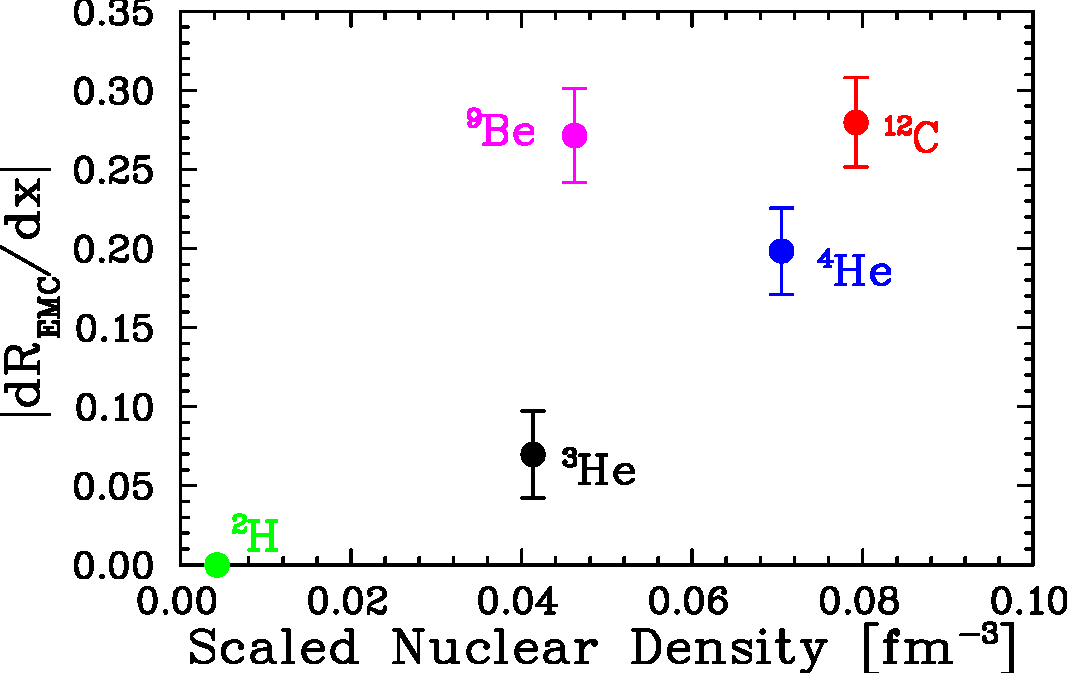
\includegraphics[width=0.5\textwidth]{plots/e03103_slopes.pdf}
  \caption{Size of the EMC effect (defined as $|dR/dx|$ between for $x=0.35-0.7$) vs. scaled nuclear
    density~\cite{Seely:2009gt}.}
  \label{fig:emc_jlab_hallc}
\end{figure}

Later, it was suggested that so-called short-range nucleon-nucleon correlations (SRCs) in nuclei also result
in high local nuclear density, and when the size of the EMC effect was plotted vs. the
$a_2=\sigma_A/\sigma_D$ ratio of
inclusive cross sections at $x>1$ (which is sensitive to the ``number of short range correlations''
found in a nucleus) a linear correlation between the two quantities was observed~\cite{Weinstein:2010rt}.
This correspondance was even more compelling when $x>1$ ratios for Be from JLab experiment E02-019 became
available and the same correlation was observed~\cite{Hen:2012fm}, Fig.~\ref{fig:emc_src_bff}.

\begin{figure}[htb]
  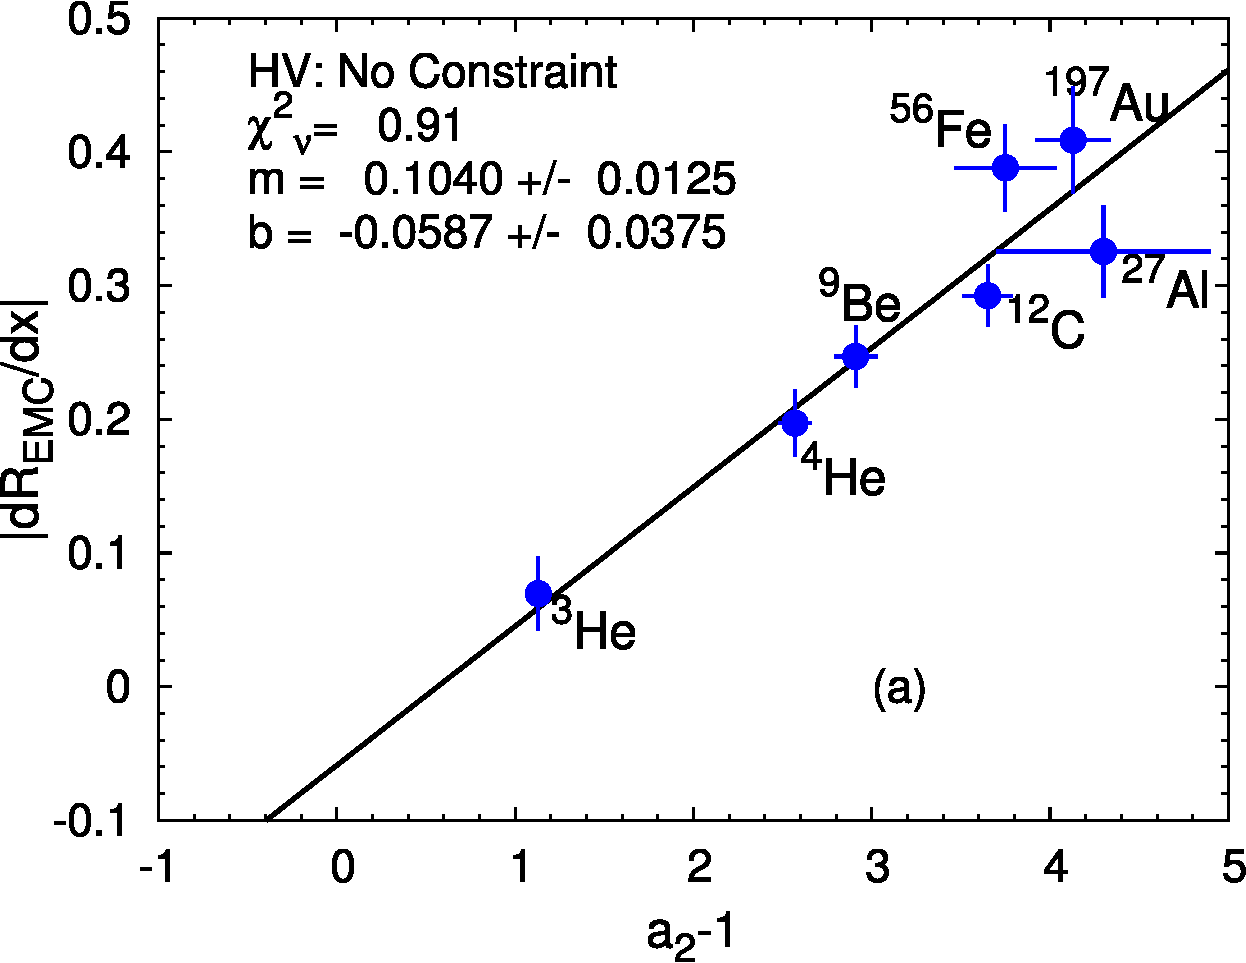
\includegraphics[width=0.5\textwidth]{plots/plotfit_all_norescaling_nocm_rean_final.pdf}
  \caption{Size of the EMC effect plotted vs. the SRC $a_2$ ratio. Data are from JLab and SLAC. Figure
  from Ref.~\cite{Arrington:2012ax}.}
  \label{fig:emc_src_bff}
\end{figure}

The origin of this correspondance is unclear, whether SRCs in some way cause the EMC effect, or if the two
phenomena are caused by some common underlying source.  A study was conducted to examine whether
both the EMC effect and SRCs are correlated with some other independent variable~\cite{Arrington:2012ax} such
as average nucleon separation energy, etc., with no clear common origin or factor found.

%\documentclass[prb,11pt]{revtex4}
%\documentclass[twocolumn]{revtex4}

%\usepackage{amsfonts, amsmath, amssymb, mathrsfs}
%\usepackage{verbatim}
%\usepackage{url}
%\usepackage[pdftex]{graphicx}           % Standard graphics package
%\renewcommand{\thefootnote}{\fnsymbol{footnote}}


%\begin{document}
\section{nPDFs in the high-x region}

Nuclear parton distributions functions (nPDFs) are the first step in understanding the behavior of nuclear matter at the elementary particle level. Moreover they play a crucial role in the determination of the free proton PDFs, as light nuclear targets are routinely used for separating the different partonic flavors in PDFs fits. Notwithstanding their importance, nPDFs are not as well known as the free proton ones, mainly due to two factors. On one side, despite the phenomenal success of HERA in determining the proton structure, no $e+A$ collider has ever existed. On the other side, only a few nuclei have been studied in detail (He, C, Fe) and the data span a limited region of the kinematic space, to the point that the only constrained nuclear distributions are the valence quarks in the mid-x region, assuming the same nuclear modification for the up and down quarks. Furthermore, the parameterizations of the nuclear effects in the neutron are done by assuming the validity of the isospin symmetry, which which is hard to test given the nearly isoscalar nature of most available nuclei.  Less than about one third of the data used in the fits come from heavy nuclei which complicates the possibility of truly separating the nuclear modifications for each flavour. A possible path for doing so would be using charged current (CC) data from DIS, available for iron and lead, as the cross-section depend on different combinations of the PDFs than the neutral current (NC) processes. It has been also suggested that nuclear effects might not be universal and therefore making a truly global fit of the nPDFs would not be possible. Up to now and within experimental uncertainties, NLO fits including NC and CC data have not shown visible tension. Unfortunately these fixed target experiments cover a very limited region of the kinematic space and are lacking in precision, not allowing yet for a conclusive answer.


 Extrapolations for $x < 10^{-3}$ obey the fulfillment of the charge and momentum sum rules and, at mid to high-$x$, the sea quarks and gluon densities are determined by ad-hoc assumptions during the fitting procedure, rather than from actual constraints from the data. 

The unexplored low-$x$ region, dominated by the gluon density, opens the possibility of finding new non-linear phenomena such saturation, and puts to test the applicability range of the linear regime. The other extreme of the kinematic space, the high-$x$ region, is of particular interest as there appears the first measured sign of nuclear effects in high energy collisions: the EMC effect. Moreover, for beyond the Standard Model searches at the LHC, rare high-$x$ gluon initiated events could be enhanced. However the nuclear gluon is difficult to access at high-$x$, and great care has to be put in its determination. Despite the lack of data, the determination of nPDFs in all the kinematic space is of crucial relevance and thus the target of several efforts. Given the fact that sea quarks and gluon densities are tied through the DGLAP evolution equations, studying processes sensitive to either sea quarks or gluons has an impact on our knowledge of nPDFs.    

%\subsection{Drell-Yan processes}

%AFTER!

\subsection{Accessing the nuclear gluon at high-x}

One of the observables in which initial state gluons can account for most of the cross-section are jets. Unfortunately the LHC measurements in jets in $p+\mathrm{Pb}$ collisions by the ATLAS collaboration~\cite{ATLAS:2014cpa} have been integrated over in the $0-90\%$ centrality bin instead of as the customary minimum bias data, rendering the quantity difficult to compare to in the context of collinear factorized pQCD. However, the data of the di-jets measured by the CMS collaboration were published~\cite{Chatrchyan:2014hqa} and further included in the latest NLO nPDF analysis of EPPS16~\cite{Eskola:2016oht}. There it was shown that, while at $Q^{2}$ where some information is lost in the PDF evolution, the di-jets have a non-negligible impact on the high-$x$ gluon distribution. As the EPPS16 fit comprises about $2000$ data points and allows for more flexible parameterizations, the effect of the di-jet data on constraining the gluon is significantly diluted. 

Nonetheless, jets remain a relevant tool to access the gluon density. In recent works~\cite{PhysRevD.95.094013, PhysRevD.97.114013} it has been shown that (di-)jets in $e+A$ collisions at a future Electron-Ion Collider (EIC) have the potential to reduce the theoretical uncertainties by an order of magnitude at both low and high-$x$, reaching into the anti-shadowing and EMC effect regions.

A complementary way of accessing the high-x gluon is using the charm quark structure function. This quantity is determined by tagging the charm in the final state and, theoretically, has its first non-zero contribution from the photon-gluon fusion process. In addition, this observable might hold the key to study if there is an intrinsic content of charm in the proton or nucleus or if heavy quarks appear only by radiation form the gluons. The studies of DIS reduced cross-section with simulated EIC data and its impact on the gluon nPDF~\cite{PhysRevD.96.114005} show that the inclusive data could reduce the uncertainty bands up to a factor of~4 at low $x$, while the charm reduced cross-section would have a dramatic effect, diminishing the uncertainties by almost an order of magnitude at high-$x$.   

%\begin{thebibliography}{5}


%\end{thebibliography}


%\end{document}




%\documentclass[prb,11pt]{revtex4}
\documentclass[twocolumn]{revtex4}

\usepackage{amsfonts, amsmath, amssymb, mathrsfs}
\usepackage{verbatim}
\usepackage{url}
\usepackage[pdftex]{graphicx}           % Standard graphics package
\renewcommand{\thefootnote}{\fnsymbol{footnote}}


\begin{document}


THIS PART, add in the first paragraph of ``NPDFS IN THE HIGH-X REGION", between ``... available nuclei." and ``Extrapolations ..."

Less about one third of the data used in the fits come from heavy nuclei which complicates the possibility of truly separating the nuclear modifications for each flavour. A possible path for doing so would be using charged current (CC) data from DIS, available for $Fe$ and $Pb$, as the cross-section depend on different combinations of the PDFs than the neutral current (NC) processes. It has been also suggested that nuclear effects might not be universal and therefore making a truly global fit of the nPDFs would not be possible. Up to now and within experimental uncertainties, NLO fits including NC and CC data have not shown visible tension. Unfortunately these fixed target experiments cover a very limited region of the kinematic space and are lacking in precision, not allowing yet for a conclusive answer. 

\subsection{Improvements for nPDFs}

Future experiments will play a key role on determining the nPDFs. One attractive feature of these is the possibility of incorporating lessons learnt from past experiments into the data extraction, publication and analysis. A simple example of this is the results from HERA. At the very beginning data were published in the form of the structure functions $F_{2}$, while in later years, and after the conclusion of data taking, new studies using the cross-sections and combining H1 and ZEUS results have become available. The realization that the structure functions were not a sensible observable to the gluon density and the adding of uncertainty due to the $F_{2}$ extraction came a long time after the nuclear fixed target experiments were finished and no re-analysis under this light have been performed. While it is true that these do not venture into the low-$x$ region, at least some increase on gluon content would be expected from using $\sigma$ instead of $F_{2}$, while removing the uncertainties coming from phenomenological parameterizations of the $F_{L}/F_{2}$ ratio. On the same page lie the corrections included into the data to account for the non-isoscalarity of some targets, that can lead to very different shapes for the EMC effect if not being considered. In this light it would be extremely beneficial for the community to publish the future results in all possible formats, i.e., the measured $\sigma$, the extracted $F_{i}$, with and without corrections, so that studies could be performed in the desired way. 

Another aspect that would be beneficial for the extraction of the nPDFs is the improvement of our understanding of final state effects. Unlike proton PDFs, where the determination of the gluon is not contaminated by final states, the nPDFs have been including routinely particle production in $d+Au$ collisions into the fits, an observable that is very sensitive to both the initial and final state (hadronization) of the gluon. This would be in principle a perfectly adequate idea, except that it has some caveats. The fragmentation functions (FFs) in the vacuum are best determined for the pions, with the gluon fragmentation having a sizable theoretical uncertainty. Moreover data from the LHC at $7$ GeV can not be well described by a global fit unless a significant cut in $p_{T}$ is applied to the date, leaving out a relevant portion of the $d+Au$ covered region. Furthermore, when it comes to particle production in a nuclear medium it is yet unclear how much of the measured effects can be attributed to the nPDFs and how much of it, if any, is a final state effect due to the partons interacting with the medium before the hadronization. The only semi-inclusive DIS off nuclei, measured at HERMES, shows a significant effect that has yet to be understood. This constitutes a sizable source of uncertainty for the extraction of the nPDFs and therefore conclusions from incorporating particle production data form RHIC into the fits must be drawn carefully.   

\begin{thebibliography}{5}


\end{thebibliography}


\end{document}




\section{Future Directions for Inclusive Unpolarized EMC Effect Measurements}

With the observation that the EMC effect may be driven by the local nuclear environment
and the apparent correspondance between the EMC Effect and short range correlations, it is worth examining what
further studies with inclusive electron scattering can shed light on the origin of the EMC Effect.

One clear avenue of exploration is to make EMC Effect measurements from additional light to medium-light
nuclei where ab-initio nuclear structure calculations are feasible and interesting nuclear cluster
structures may manifest.

Additionally, one can leverage the fact that SRCs are dominated by neutron-proton pairs to further explore
the robustness of the EMC-SRC correlation by measuring the EMC Effect for a range of nuclei with
different neutron to proton ($N/P$) ratio at fixed $A$, and for a range of $A$ at fixed $N/P$.

Both of the above will be accomplished by JLab experiment E12-10-008~\cite{12gev_emc} in combination
with E12-06-105~\cite{12gev_xgt1}. E12-10-008 will measure the EMC Effect for a wide range of nuclei,
aimed at elucidating the EMC-SRC connection, providing first measurements for a variety of light nuclei,
and exploring in-medium $n/p$ ratios via measurements of $A$ and $A\pm1$ nuclei.  E12-06-105 will make
measurements at $x>1$ in the two-nucleon correlation region for the same nuclei as well as make additional
measurements in search of possible three-nucleon correlations. Figure~\ref{fig:np_ratios} shows the $N/P$
ratio against $A$ for the nuclear targets that will be used for both experiments.

\begin{figure}[htb]
  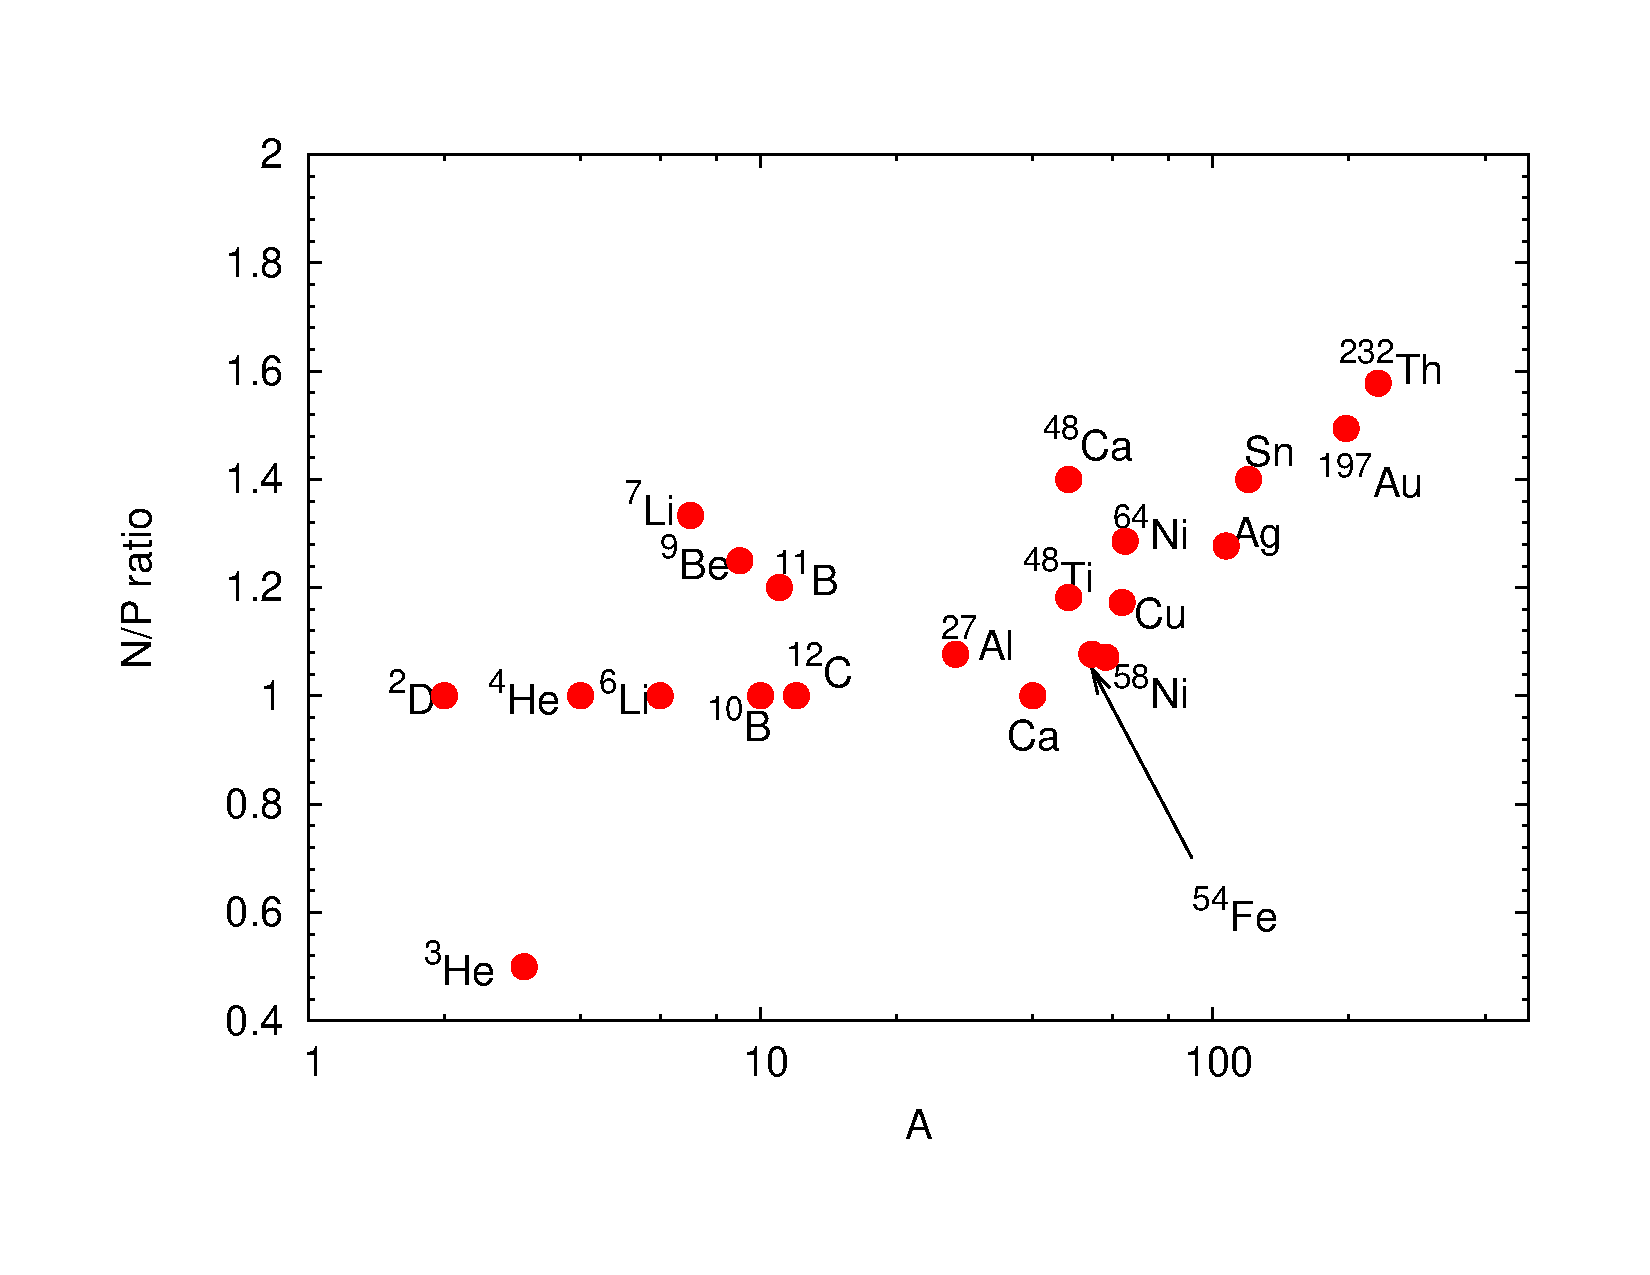
\includegraphics[width=0.5\textwidth]{plots/np_ratios_2017.pdf}
  \caption{$N/P$ ratio vs. $A$ for nuclei that will be measured by JLab experiments E12-10-008 (EMC Effect)
    and E12-06-105 ($x>1$) to further elucidate the apparent link between the EMC Effect and short range
    correlations.}
  \label{fig:np_ratios}
\end{figure}

\section{Isovector EMC Effects}

One aspect of the EMC effect that has not been fully explored are isovector-dependent effects.  Such effects would necessarily include degrees of freedom beyond the nuclear mass number $A$, which as has long been a method of parameterization~\cite{Malace:2014uea}.  In this situation, the nuclear $u_A$ and $d_A$ distributions can be modified separately, for example in an isovector mean field background or due to a preference in nucleon flavors in short range correlation pairing.  In a flavor separation which makes the assumption that $u_p = d_n$ and $d_p = u_n$ in the modified system, this manifests itself as an apparent charge symmetry breaking, though only by the assumption that protons and neutrons retain their local charge symmetry identity.  This is assumption is not necessarily true for a bound system and can be invalid for asymmetric nuclei in the same vein as the binding energy has a symmetry energy component.  Under the binding energy argument, as the symmetry energy is subleading to other bulk effects, such an isovector effect would be sub-leading to isoscalar modification effects.

The present world data have poor constraints on such an effect, in particular because many measurements of the EMC effect use symmetric or weakly asymmetric nuclei.  One calculation~\cite{Cloet:2009qs} using the Nambu-Jona-Lasinio (NJL) model and including the nuclear symmetry energy as an input, predicts deviations from the isoscalar EMC effect in the parton distribution functions on the order of several percent.   

Calculations based on short ranged correlations predict a similar picture~\cite{Sargsian:2012sm}.  The observed correspondence of the short range correlation plateau with the slope of the EMC effect would indicate local densities as a driving mechanism~\cite{PhysRevLett.106.052301}.  Using the observation that proton-neutron pairs are found much more frequently than neutron-neutron or proton-proton pairs~\cite{Subedi:2008zz} and simple counting arguments, modification of protons and neutrons will be different in nuclei depending on the asymmetry.  In either a mean field or short ranged correlation model, observation in the difference of quark flavors would require very high precision electromagnetic deep inelastic scattering measurements due to the suppression of the $d$ quark components by the square of the charges. 

Weak interactions offer a novel method to probe for these types of effects.  In charged-current processes, $u$ and $d$ quarks only participate in $W^-$ or $W^+$ exchange respectively and could be used to map out the flavor dependence.  The NuTeV experiment~\cite{Zeller:2001hh} was carried out using neutrino beams at Fermilab using the Paschos-Wolfenstein relation~\cite{Paschos:1972kj} to measure the weak mixing angle, $\sin^2\theta_\mathrm{W}$.  Due to the small neutrino cross section, heavy targets (iron) were employed which have a small neutron excess.  Charge symmetry in the bound nucleons was assumed and a significant deviation in $\sin^2\theta_\mathrm{W}$ was observed.  With the inclusion of an effect predicted by the NJL calculation noted above, much of the deviation is resolved.  Additionally, tension has been noted in nuclear PDF fits between neutrino data and other data sets which probe different flavor combinations~\cite{Schienbein:2009kk}.

\subsection{Flavor Dependence with Parity Violation}

The interference between electromagnetic and  neutral currents through parity-violating deep inelastic scattering can be used as a more precise measurement than available in electromagnetic scattering~\cite{Cloet:2012td}.  In this situation, a polarized lepton beam scattered from an unpolarized asymmetric nuclear target will form a small parity-violating cross section between the two beam helicity states, $\sigma_{\mathrm{L,R}}$, which is to leading order
\begin{equation}
        \frac{ \sigma_R - \sigma_L }{\sigma_R + \sigma_L} = -\frac{G_F Q^2}{4 \sqrt{2} \pi \alpha} \left[ Y_1 a_1(x) + Y_3(y) a_3(x) \right],
            \label{eq:phy:apv}
\end{equation}
where $G_F$ is the Fermi constant, $\alpha$ the fine structure constant, $x=Q^2/(2M\nu)$ the standard Bjorken-$x$ variable, $M$ the mass the of nucleon, $\nu$ the lepton energy transfer, and
\begin{equation}
        Y_1 \approx 1; \qquad Y_3(y) \approx \frac{1 - (1-y)^2}{1 + (1-y)^2}
    \end{equation}
    with
    \begin{eqnarray}
            a_1(x) & = &  2 \frac{ \sum_i C_{1i} e_i (q_i + \bar{q}_i) }{ \sum_i e_i^2 (q_i + \bar{q}_i) } \\
            a_3(x) & = &  2 \frac{ \sum_i C_{2i} e_i (q_i - \bar{q}_i) }{ \sum_i e_i^2 (q_i + \bar{q}_i) }. 
    \end{eqnarray}
    with $y=\nu/E$,  $E$ the beam energy, $e_i$ the quark electric charge couplings for flavor $i$, and $C_{1i}$ and $C_{2i}$ the effective quark couplings dependent on the weak-mixing angle $\sin^2\theta_\mathrm{W}$~\cite{Patrignani:2016xqp}.  The $a_1(x)$ term is dominant for fixed target, forward angle kinematics with $C_{1u} \approx -0.19$ and $C_{1d} \approx 0.34$.  An experimental proposal~\cite{emcpvdis} for the proposed SoLID spectrometer at JLab would be able to test the difference between an NJL-sized effect and naive effect to better than 5-$\sigma$ using a ${}^{48}$Ca target, Fig.~\ref{fig:ivemc:pvdis}.

    \begin{figure}
        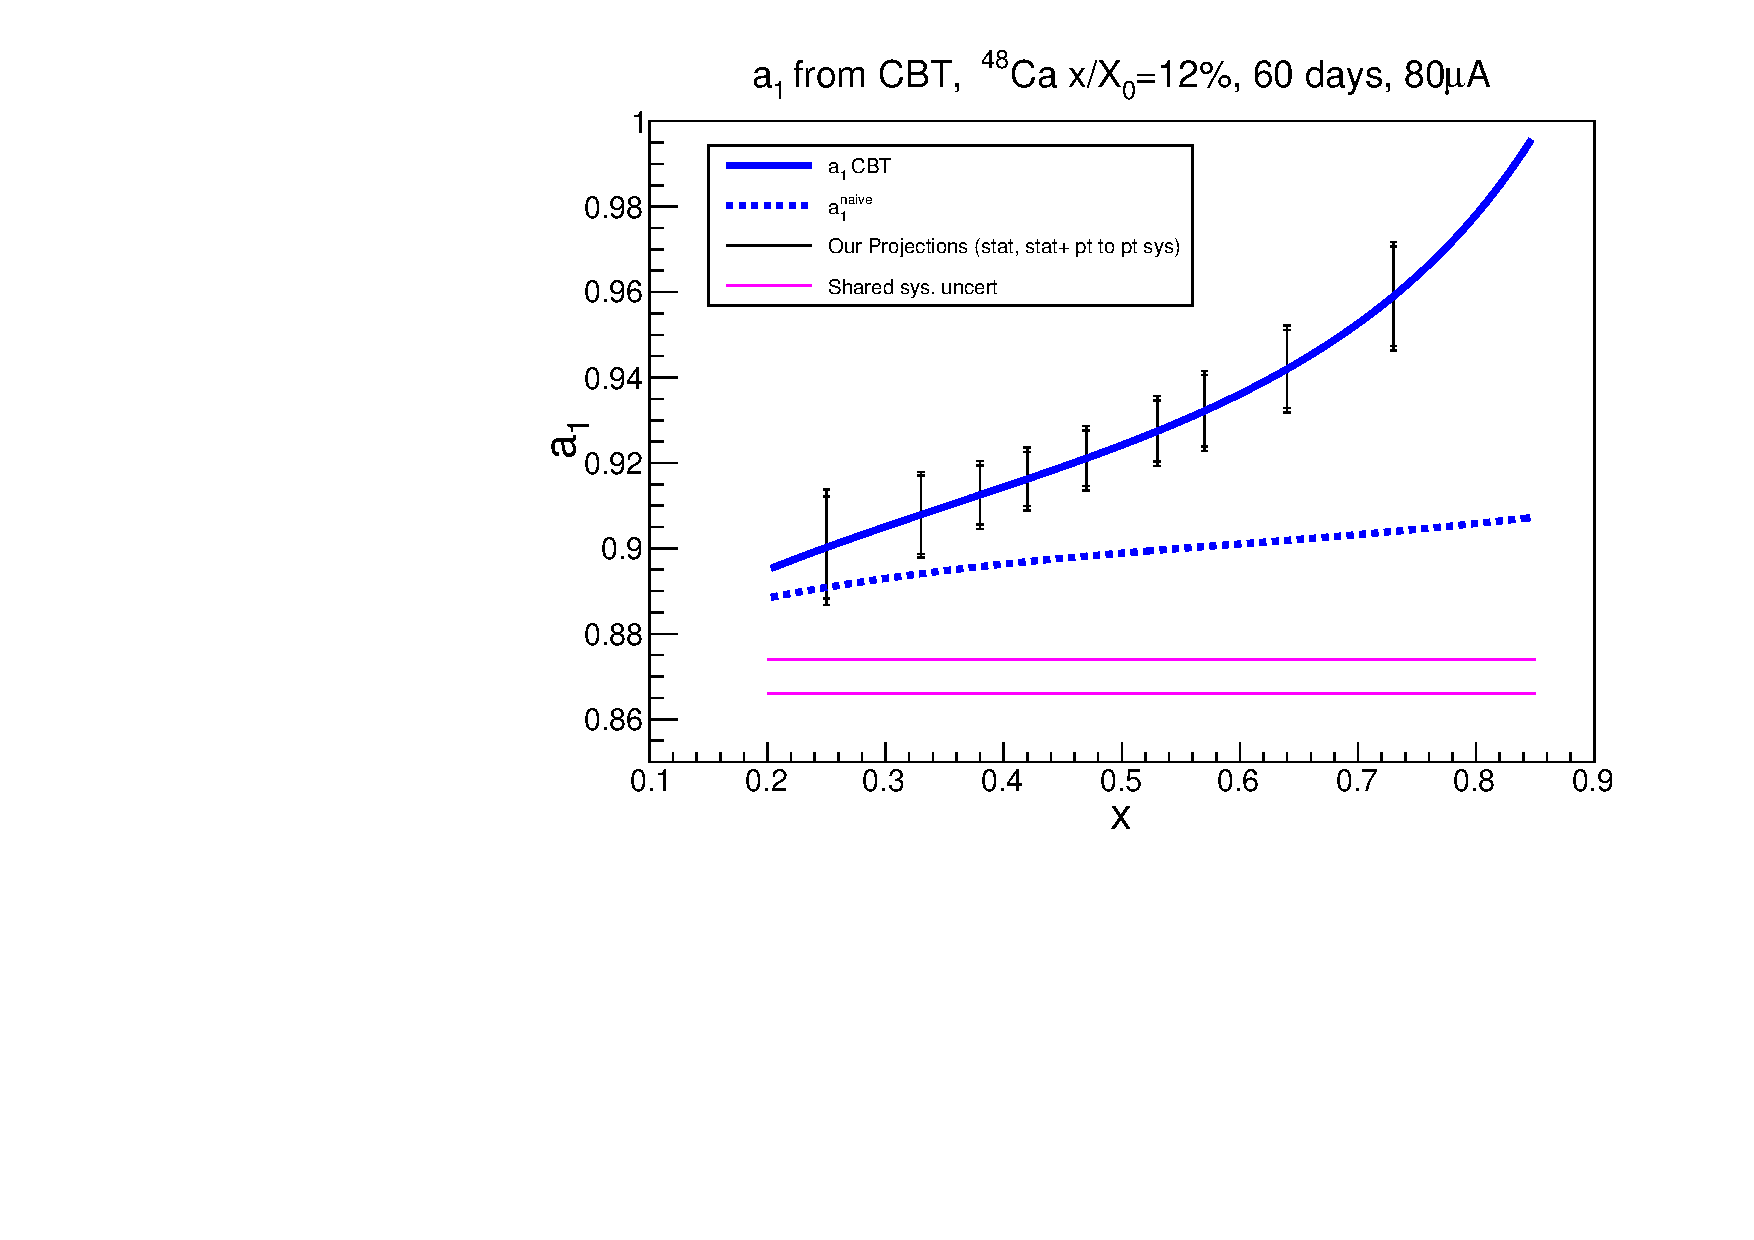
\includegraphics[width=0.5\textwidth]{plots/a1proj_2016.pdf}
        \caption{Projected sensitivities of the quantity $a_1$ for a proposed parity-violating deep inelastic scattering experiment~\cite{emcpvdis}.}
        \label{fig:ivemc:pvdis}
    \end{figure}






\section{Spin Dependent EMC Effect}

Ever since its discovery~\cite{Aubert:1983xm,Bodek:1983ec}, it has been clear that the EMC 
effect~\cite{Geesaman:1995yd} embodies important new information about nuclear structure. Unfortunately, the information is so well encoded that there is as yet no consensus on what it is telling us. It has been argued forcefully (see for example Ref.~\cite{Thomas:2016bxx,Guichon:2018uew}) that the model independent fact that there is a very strongly attractive scalar mean field in nuclei leads to changes in the internal structure of bound nucleons that can not only explain the EMC effect but play a vital role in the binding of atomic nuclei~\cite{Stone:2017oqt,Stone:2016qmi}. 
%
    \begin{figure}[h!]
        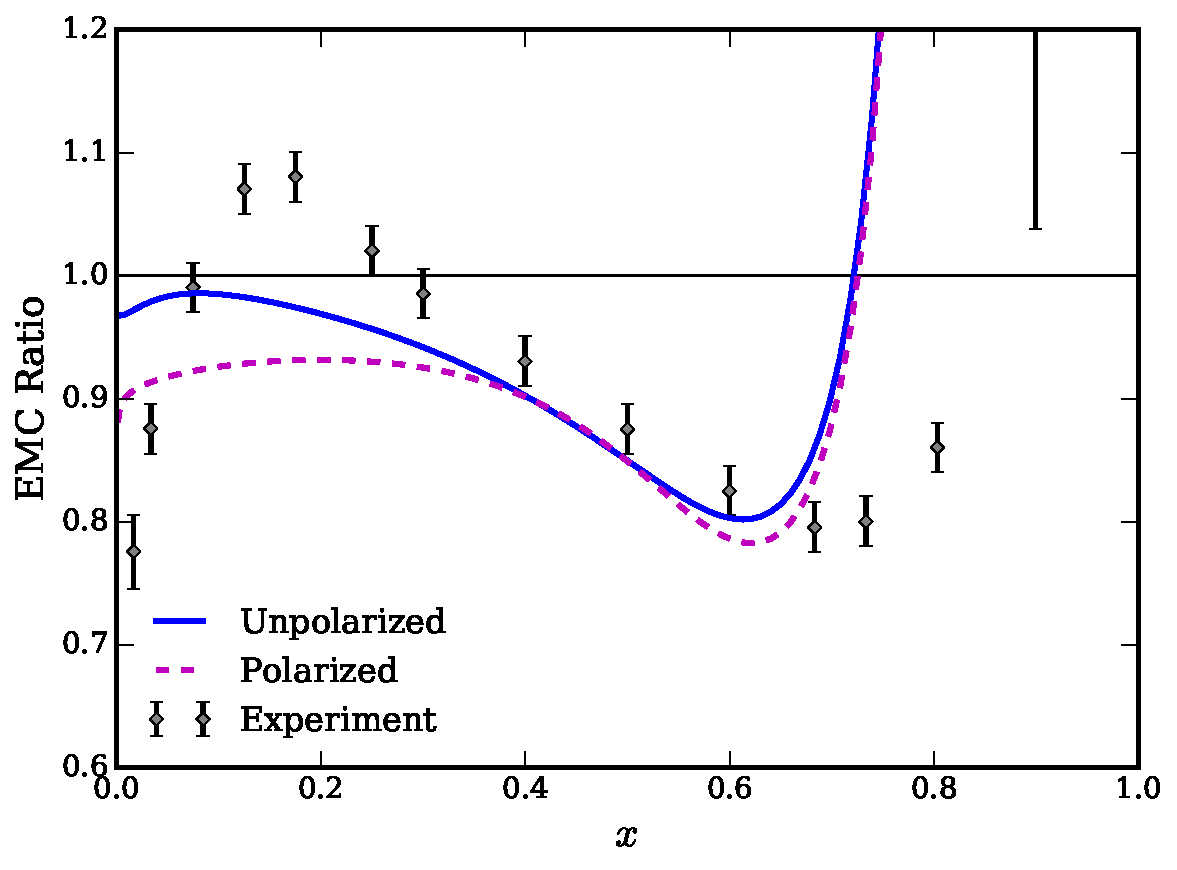
\includegraphics[width=0.5\textwidth]{plots/EMC_Com_NLO_PDF.pdf}
        \caption{Unpolarized and polarized EMC effect in the QMC model. The results are evolved to $Q^2=10$ GeV$^2$. The EMC data for nuclear matter is taken from Ref.~\cite{Sick:1992pw}.}
	\label{fig:EMC_Com}
    \end{figure}
%

In order to distinguish between the various proposals that have been made by way of explanation for the EMC effect it is vital to find new observables which may shed light on which is correct. %Within a mean field approach, based upon the NJL model~\cite{Bentz:2001vc}, it was suggested that the isovector mean field in a nucleus with $N \neq Z$ would give rise to an isovector EMC effect~\cite{Cloet:2009qs,Bentz:2009yy}. In practice such an effect acts like an effective increase in the charge symmetry violation which is already present in nucleon PDFs because $m_d \neq m_u$~\cite{Londergan:2009kj} and leads to a substantial correction to the supposed NuTeV anomaly~\cite{Cloet:2009qs,Bentz:2009yy}.  A number of important proposals involving parity violating deep inelastic scattering have been made at Jefferson Lab which could clearly identify this novel aspect of the EMC effect~\cite{Cloet:2012td}.

Here we focus on the proposal of Clo\"et {\it et al.}~\cite{Cloet:2005rt,Cloet:2006bq} that it would be interesting to measure the modification of the polarized structure function of a bound proton. These investigators first studied the hypothetical case of the structure structure function, $g_1^p$, of a proton bound in nuclear matter.  The bound proton was assumed to be 100\% polarized and the effect of the medium was dramatic. The EMC effect was roughly twice as large for the spin dependent case as for the unpolarized case.  For comparison, if one were to take the extreme position that all of the EMC effect arises from high momentum (highly correlated) nucleons~\cite{Weinstein:2010rt}, it seems unlikely that there would be any effect on the spin structure function.

Strangely, even though the first calculation of the EMC effect within a self-consistent treatment of the modified structure of a bound nucleon was carried out 30 years ago~\cite{Thomas:1989vt}, there has so far 
been no calculation of the spin dependent EMC effect within that model -- the 
QMC model~\cite{Guichon:1995ue}. This is now of particular interest because it has been possible to derive an energy density functional equivalent to the QMC model, which starts with the modification of the quark structure of the nucleon in-medium, which has proven rather effective in nuclear structure studies~\cite{Guichon:2018uew,Stone:2017oqt,Stone:2016qmi}. 

A calculation of the polarized EMC effect was recently carried out within the QMC model by 
Tronchin {\it et al.}~\cite{Tronchin:2018mvu} and from the result shown in Fig.~\ref{fig:EMC_Com}, which is taken from that paper, we see that the prediction of the polarized EMC effect in the QMC model is about the same as that of the unpolarized effect.  We stress that this polarized EMC effect is defined for a proton which is 100\% polarized. In a real nucleus, such as $^7$Li, for which a measurement is planned at Jefferson Lab~\cite{JLab}, one needs to account for the fact that the polarization of the bound proton is less than that of the nucleus. 





\section{Drell-Yan and Nuclear PDFs}

Most of our knowledge on the medium-modified PDFs come from DIS experiments. Although extensive and precise, 
these data are not able to independently investigate the nuclear effects on sea and valence quarks.  
Moreover, they do not discriminate between the different flavors participating in the reaction. Finally, 
they do not probe the nuclear gluon distributions. Additional studies of the effect of the medium on the 
PDFs can be provided by dedicated fixed-target dimuon production experiments. In the Drell-Yan mass region
 these experiments can be used to isolate  
valence and sea distributions as well as to separate the two light flavors of the quark PDFs. 
The unknown gluon distributions in nuclei can be accessed by analyzing the contributions to  
the charmonium production cross-sections. 
 
\subsection {Valence quark distributions and the EMC effect}
Only a few Drell-Yan experiments have investigated the medium modifications in nuclear targets. 
The Drell-Yan data from the E772 experiment~\cite{Alde:1990im} show no visible nuclear effects in 
the anti-shadowing domain, both E772 and E866 experiments~\cite{Vasilev:1999fa} are compatible 
with the DIS data in the onset of the shadowing region, Fig.~\ref{fig:drell-yan}.  An exploration of the medium effects for larger $x$ 
values was recently completed by the SeaQuest experiment~\cite{seaquest} at Fermilab. 

\begin{center}
\begin{figure}[htb]
  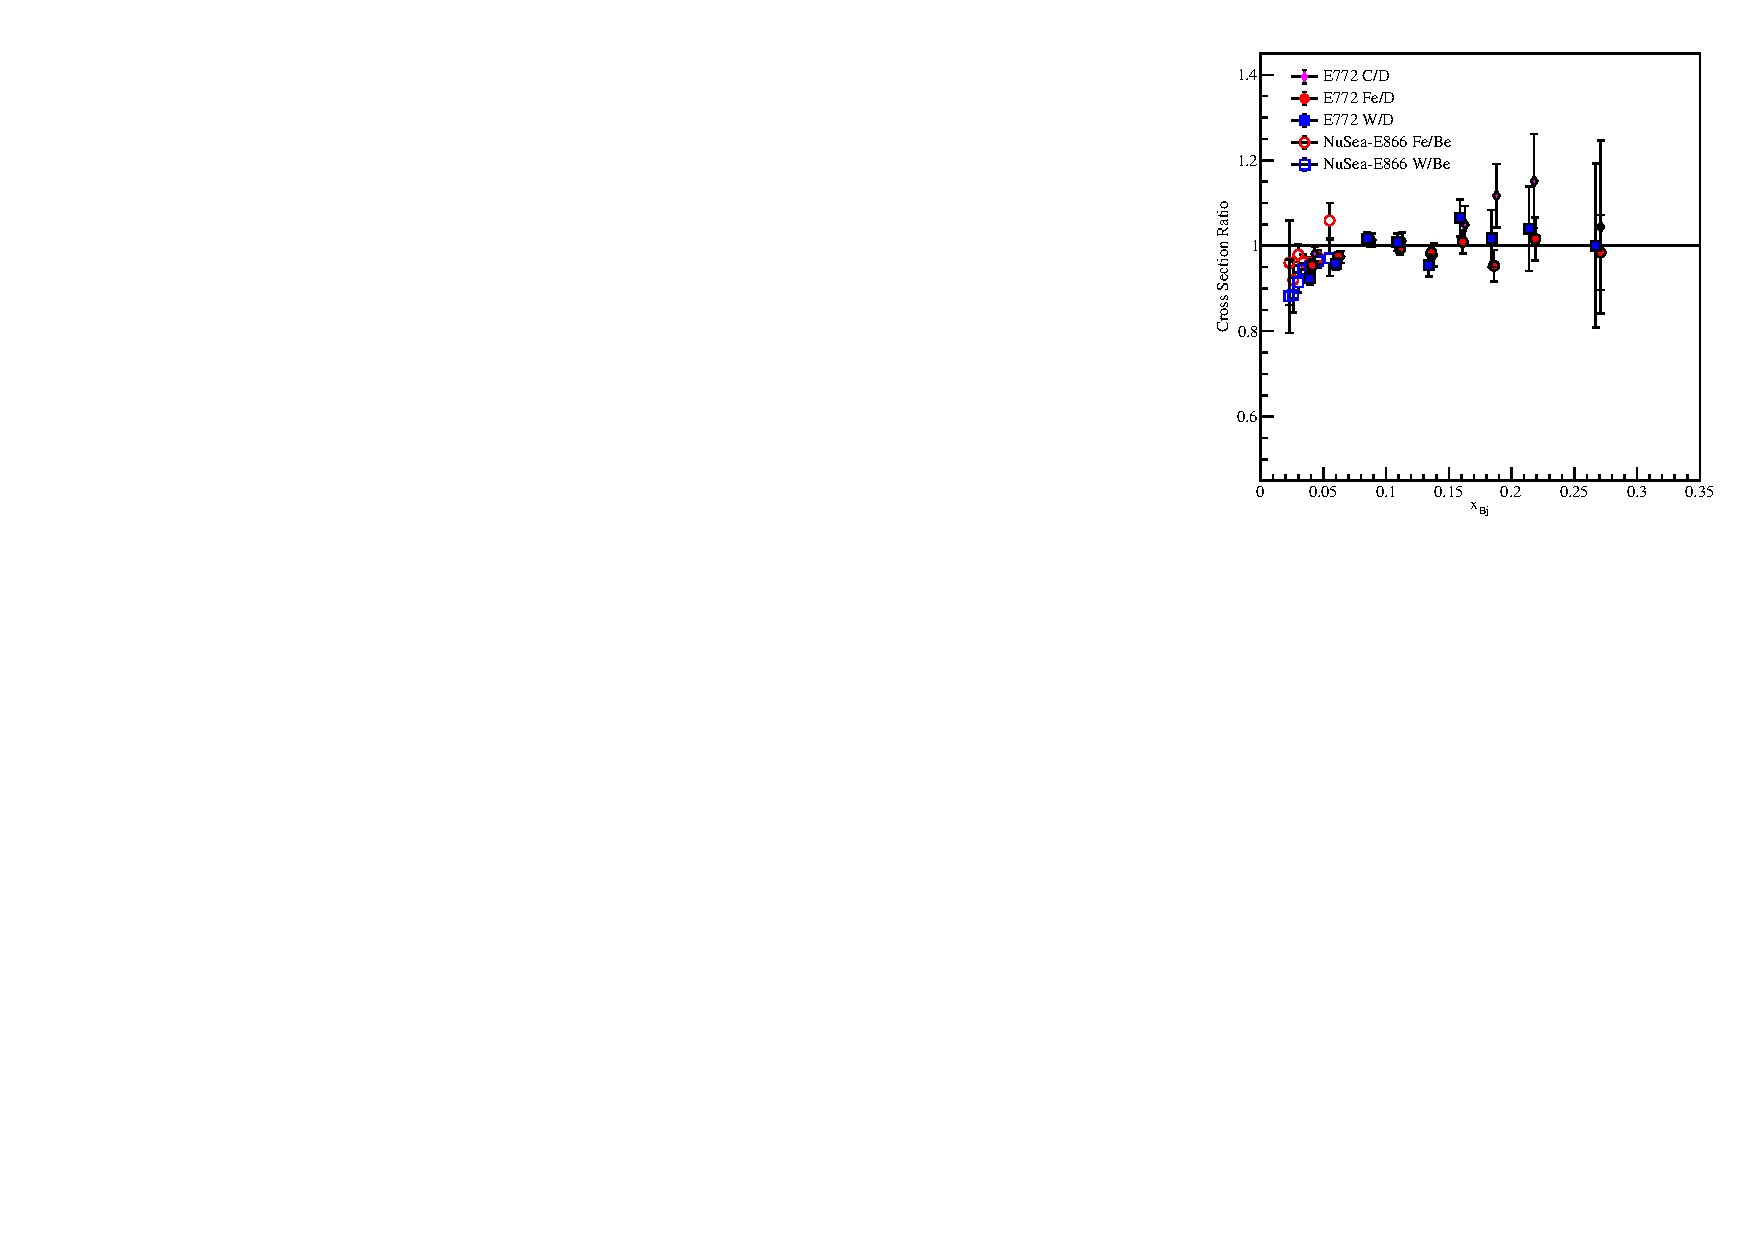
\includegraphics[width=0.45\textwidth]{plots/Drell-Yan_EMC.pdf}
  \caption{Drell-Yan cross section ratios from E772 and E866 \cite{Alde:1990im, Vasilev:1999fa}.}
  \label{fig:drell-yan}
\end{figure}
\end{center}


All these experiments use proton beams. They are mainly sensitive to the antiquark 
distributions in nuclei.  Since pions contain also valence antiquarks, pion beams are  
an ideal tool for the investigation of the valence quark distributions. Pion-induced Drell-Yan data have 
been taken in the past by two CERN experiments, NA3~\cite{Badier:1981ci} 
and NA10~\cite{Bordalo:1987cs}.  For both experiments the achieved statistics is limited
and the conclusions of the authors inconsistent.  

A dedicated Drell-Yan experiment, 
combining nuclear and deuterium targets could significantly improve the results. 
A high-intensity pion beam with incident momenta between 100 and 200 GeV/$c$ is presently available 
only at CERN. Since in Drell-Yan experiments the total cross section increases with the energy, a higher 
energy is preferable. On the other hand, a maximal coverage of the high-$x$ EMC could require a 
lower incident momentum.  

\subsection{Flavor dependence of the EMC effect} 
%The flavor dependence of the nuclear mean field was recently investigated~\cite{Cloet:2009qs} using a 
%covariant Nambu-Jona-Lasinio (NJL) model.  The main conclusion of this study is that for nuclei with 
%N$>$Z, the isovector-vector mean field affects differently the two lightest quark distributions,
%causing an additional attraction (repulsion) for the $u$ and $d$ quarks respectively. 
%This additional vector field modifies differently the corresponding nuclear PDFs, resulting in an effect of 
%the medium which is more than twice larger for the $u$ quarks. An experimental evidence of this flavor 
%dependence is still missing. 

The sensitivity of the available Drell-Yan data on the flavor-dependent effect was explored in 
Ref.~\cite{Dutta:2010pg}. A comparison with calculations based on the model of Ref.~\cite{Cloet:2009qs} 
shows that the  statistics of the available data~\cite{Badier:1981ci,Bordalo:1987cs} is insufficient to draw firm conclusions. 
The flavor dependence may also have an effect 
on the global nuclear PDF fits presently available. Indeed, when releasing the flavor constraints in these fits, 
the model uncertainties increase~\cite{Paakkinen:2016wxk} by a large factor. 

The effect coming from the flavor dependence of the mean field can be further amplified by 
comparing positive and negative pion beam Drell-Yan data on the same heavy target. Negative pions probe mainly the 
target $u$-valence quarks, whereas positive pions prefer $d$-valence quarks. Pion beams of both charges
are presently available only at CERN. 

\subsection{Nuclear dependence of the gluon distribution}

The effect of the nuclear mean field on the gluon distribution is presently unknown. Available nuclear PDFs produce 
very different results~\cite{Cazaroto:2008qh} in the whole region of $x$ and particularly for $x > 0.1$.
The J/$\psi$ production data, 
usually collected in parallel with Drell-Yan data, can be used as a probe of the nuclear gluon distributions. 
The production of J/$\psi$ proceeds through either the $q\bar q$ or the $gg$ fusion processes, the $gg$ 
contribution being the dominant one~\cite{Vogt:1999dw} for $x_F < 0.5$  even at low center-of-mass energies. 

As for Drell-Yan, most of the J/$\psi$ production data were taken with proton beams. The nuclear dependence 
was primarily used for the evaluation of the absorption of the J/$\psi$ as a function of the atomic number. 
Pion-induced J/$\psi$ data have been taken by several experiments, but most of the time with a single target. 
A comparison of several nuclear targets (Si, Cu, W) was also made~\cite{Alexandrov:1999ch},  
but unfortunately for the total cross-sections only. High-statistics J/$\psi$ production data on   
the $x$ dependence, combining nuclear and light targets, are still missing. 

The strong-interaction J/$\psi$ production process has one important advantage: its cross-section is large, 
Large statistics J/$\psi$ production data can be collected and 
used to precisely map out the $x$-dependence of the nuclear modifications. Such data could be 
used for a better assessment of the charmonium production process.  The gluon distributions could 
therefore be inferred with minimized model-dependence uncertainties.  


\section{Opportunities with low $A$ nuclei}

The primary difficulties of modeling nuclei within the QCD framework are the
strong coupling constant which does not lend itself to perturbative calculations
and the further complication of a many body system.  Presently, 
even the most advanced
techniques are only able to approach descriptions of nuclei with $A \le 4$, 
which is below where one may expect bulk modification effect to occur.  However,
to ultimately obtain a full description, advancement in models and comparison
to few-body nuclear data are critical.  In addition, the formalism of generalized
parton distributions can be extended to nuclei,  offering a new window of 
exploration unifying the study of the modification of partons and form factors
and an opportunity to provide a tomographic map of nuclei.


\subsection{Opportunities with the deuteron}

The deuteron is the lightest non-trivial nucleus and it has a wave function dominated by a loosely bound proton--neutron configuration.  As such, it offers a range of possibilities to study QCD phenomena at hadronic and partonic scales.  As it offers a (bound) neutron target, DIS off a deuteron is together with PVDIS the main tool to perform flavor separation of quark distribution functions.  As a bound $pn$ system, it also offers a window into the QCD origin of the nucleon-nucleon force and medium modifications of nucleon properties~\cite{Boeglin:2015cha}.  In kinematics where a high-energy probe interacts with both nucleons in the deuteron, coherent phenomena in QCD such as shadowing and saturation can be studied.  Lastly, the deuteron is a spin-1 hadron and as a result studies with a polarized deuteron offer additional observables and opportunities beyond those of the free polarized nucleon.

When inclusive DIS is carried out on a nucleus, the process averages over all initial configurations.  This means one has to account for possible medium modifications and include binding effects and non-nucleonic degrees of freedom in the nuclear wave function.  A handle on the control of the initial state of the target nucleus is provided by the spectator tagging process, where a slow nucleon (relative to the center of mass of the nucleus) is detected in the target fragmentation region of the final state.  For the deuteron, controlling the initial target state through spectator tagging has several advantages.  Spectator tagging effectively identifies the active nucleon participating in the DIS reaction (proton tagging enables neutron structure studies and the other way around) and suppresses nuclear binding effects at low spectator momenta. 

By varying the momentum of the detected spectator, one can also select compact (high momentum) or loose configurations (low momentum) of the deuteron (see Fig.~\ref{fig:size}).  This allows the study of nuclear binding effects and the nature of the $NN$-interaction at different length scales and densities.  Of course, one has to account for the possible final-state interactions (FSIs) between the spectator and the DIS products.  The deuteron has the advantage there is only one possible spectator nucleon, meaning FSIs are tractable.  Moreover, in kinematics with large FSIs they can be used to obtain information about the process of hadronization in the DIS products~\cite{Cosyn:2017ekf}.  

The deuteron also has the advantage that first principles non-relativistic wave functions are available to perform theoretical calculations.  In high-energy reactions, the structure of the light-front deuteron wave function is known~\cite{Frankfurt:1981mk,Keister:1991sb} and it can be matched to the non-relativistic wave functions at small relative momenta.

    \begin{figure}
        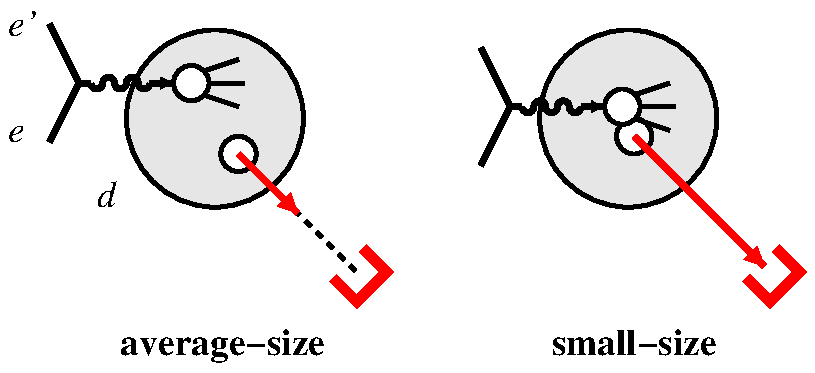
\includegraphics[width=0.5\textwidth]{plots/deut_tag_restframe}
        \caption{Deuteron lab frame depiction of the spectator tagging process.  Low spectator momenta select average-sized configurations, large spectator momenta access small-sized ones~\cite{deutLDRD}}
        \label{fig:size}
    \end{figure}

To access on-shell nucleon structure, the technique of pole extrapolation can be applied to the spectator tagging process.  Here, observables as a function of spectator momentum are extrapolated in the unphysical region to the on-shell point of the active nucleon.  The small binding of the deuteron implies the extrapolation length into the unphysical region is quite small, resulting in controllable errors on the extrapolated values.  The no-loop theorem implies that although higher order diagrams (suchs as FSIs) contribute to the spectator tagging process, they do not contribute at the on-shell point~\cite{Sargsian:2005rm} implying the access to free neutron structure functions for proton tagging.  Additionally, at the on-shell point the deuteron polarization is almost 100\% transferred to both nucleons due to the deuteron $S$-wave dominance, enabling the extraction of on-shell neutron spin structure in spectator tagging with polarized beams.  

Spectator tagging on the deuteron has been measured at JLab at both high (DEEPS experiment~\cite{Klimenko:2005zz}) and low spectator momenta (BoNuS experiment~\cite{Baillie:2011za}). In a fixed target setup this measurement is challenging, especially at low spectator momenta. Hence a dedicated detector had to be installed in the BoNuS experiment.  These difficulties disappear for an electron-ion collider, where the spectators still move forward after the DIS event with momenta of the order of half the deuteron beam momentum, and can be detected in forward detectors (see Fig.~\ref{fig:collider}).  Together with the wide kinematic range in Bjorken $x$ and $Q^2$ that an EIC offers, spectator tagging can make a significant impact on on-shell neutron structure data and studies of medium modifications.  Extensions of the tagging process are also possible using light nuclei beams beyond the deuteron and measuring more exclusive channels.  The theoretical framework and simulation tools for the spectator tagging process are under active development~\cite{deutLDRD,Guzey:2014jva,Cosyn:2016oiq} and estimates for the size of FSIs at an EIC have recently been provided~\cite{Strikman:2017koc}.

    \begin{figure}
        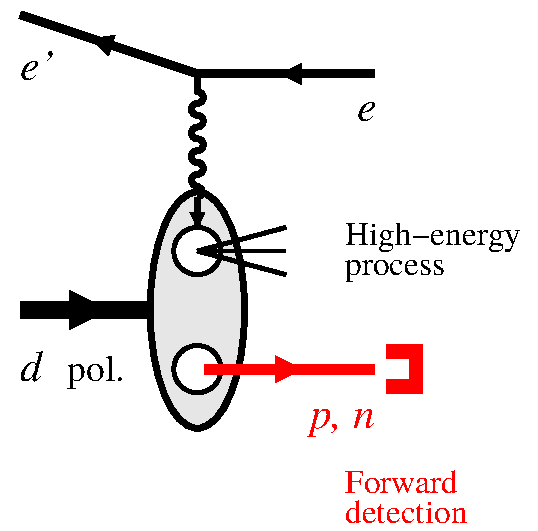
\includegraphics[width=0.28\textwidth]{plots/deut_tag_collider}
        \caption{Collider frame depiction of the spectator tagging process with forward detectors capturing the spectator nucleon~\cite{deutLDRD}}
        \label{fig:collider}
    \end{figure}

A straightforward way of probing the additional spin degrees of freedom the deuteron offers is by performing inclusive DIS off a tensor polarized target, which is sensitive to four additional structure functions~\cite{Hoodbhoy:1988am}.  One of these $b_1$ has an interpretation in the parton model as a linear combination of unpolarized quark PDFs in a polarized spin-1 hadron
\begin{equation}
b_1=\frac{1}{2}\sum_q e_q^2(q^0-q^1)\,,
\end{equation}
where $q^i$ is the quark PDF in a hadron with polarization $i$ along the virtual photon momentum.  Hence, $b_1$ probes the interplay of nuclear and quark degrees of freedom.  Currently, there exists only one measurement of $b_1$ from HERMES~\cite{Airapetian:2005cb} that cannot be explained by conventional deuteron convolution models.  A new measurement is planned at JLab~\cite{Slifer:2013vma}, which spurred updated convolution model calculations~\cite{Cosyn:2017fbo} and estimates of hidden color and pion cloud contributions~\cite{Miller:2013hla}.

\subsection{Poincar\'e Covariant Light-Front Spectral Function and Nuclear Structure}
{The Poincar\'e covariant spin-dependent spectral function, proposed in \cite{PhysRevC.95.014001, Pace:2013bq,Scopetta:2014yoa, Pace:2016eiq} and based on  the light-front (LF) Hamiltonian dynamics \cite{Dirac:1949cp, Keister:1991sb},  is a useful tool for a correct relativistic treatment  of nuclear structure, suitable for the study of deep inelastic scattering (DIS) or semi-inclusive deep inelastic scattering (SIDIS) processes at high momentum transfer \cite{mar,sid1,sid2}.}
 {Indeed the Bakamjian-Thomas construction \cite{Bakamjian:1953kh} of the Poincar\'e generators 
  allows one to embed the successful phenomenology for few-nucleon systems in a
Poincar\'e covariant framework.}

The LF spectral function, ${{\cal P}^{\tau}_{{\cal M},\sigma'\sigma}({ \tilde {\bm \kappa}},\epsilon,S)}$,
for a three-fermion system with polarization $S$ (as the $^3\mathrm{He}$ or a nucleon in valence approximation) is built up from the overlaps $_{LF}\langle  \tau T ; 
\alpha,\epsilon ;J J_{z}; \tau\sigma,\tilde{\bm \kappa}|\Psi_{0}; S T_z \rangle$, where $|\Psi_{0}; S T_z \rangle$ is the ground eigenstate of a proper mass operator \cite{PhysRevC.95.014001, Pace:2013bq,Scopetta:2014yoa, Pace:2016eiq} and 
$|\tilde{\bm \kappa}, \sigma \tau; J_{} J_{z}; \epsilon,\alpha;T \tau \rangle_{LF}$ is the tensor product of a plane wave for particle 1 with LF momentum $~ \tilde{\bm \kappa} \equiv (\tilde{\kappa}^+,{\tilde{\bm \kappa}_\perp})$ in the {{intrinsic reference frame of the $[1+(23)]$ cluster}} 
 times the fully interacting  state for {the} $(23)$ pair with  energy eigenvalue $\epsilon$.
  %As shown by {{Keister and Polyzou}} such a state {{fulfills the macrocausality}}
{{The use of the nucleon momentum {{${\tilde{\bm \kappa}}$}}
% in the intrinsic reference frame of the cluster (1,23) and the use  
%for the calculation of the LF spectral function 
%of  the tensor product of a plane  wave of momentum
%$\bm \kappa$ times the state of 
   %a fully interacting spectator subsystem 
   allows one  to take care of macrocausality \cite{Keister:1991sb} and  to introduce 
   {{a new effect of binding in the spectral function.}}}}
  % \\
% \vspace{1mm}
%\item {
%\Red 
%We have evaluated the Nucleon Spectral function
% for $^3He$, by approximating the IF overlaps with their non
% relativistic counterpart calculated  with the Av18 NN interaction}

{ As shown in \cite{PhysRevC.95.014001, Pace:2013bq,Scopetta:2014yoa, Pace:2016eiq}, the LF
% spin-dependent 
 spectral function  
%for a spin $1/2$ system composed by three fermions 
fulfills {normalization and momentum sum rule  at the same time. Integration of the spectral function on the energy 
$\epsilon$ 
of the pair yields the LF spin-dependent momentum distribution that
can  be expressed through 7 scalar functions ~~ {{${b}_{i,{\cal M}}\left [ |{\bf k}_{\perp}|,x,({\bf  S}\cdot \hat {\bf k}_{\perp})^2,({\bf  S} \cdot {\hat z})^2 \right] $}}} ($i=0,6$), straightforwardly obtained from the system LF wave function as integrals on the relative momentum, $k_{23}$, of the pair.
%\\
%An analogous expression occurs for the spin-dependent momentum distribution in terms of seven %functions ~~{{{${b}_{i,{\cal M}}\left [ |{\bf k}_{\perp}|,x, ({\bf  S}\cdot \hat {\bf k}_{\perp})^2,({\bf  S} \cdot %{\hat z})^2 \right] $}}}.
%\item
%\vspace{1mm}

{{Calculations of DIS 
%or SIDIS
 processes  based on our spectral function could indicate which is the gap with respect to the experimental data to be filled by effects of non-nucleonic degrees of freedom or by modifications of nucleon structure in nuclei.}}
%\subsubsection{EMC effect in {$^3$He} }
 {A first test of our approach is the EMC effect for $^3\mathrm{He}$.} 

 In Fig.~\ref{fig:pace} the ratio $R_2^{^3\mathrm{He}}/R_2^D$ is shown, with $R_2^A = A~ F_2^A/[Z ~F_2^p + (A-Z)~F_2^n]$.
The  spectral function has been obtained from the non-relativistic wave function  with the Av18 NN interaction of \cite{Kievsky:1997bg}. As a first step, only
%the full expression for 
the 2-body contribution 
to the spectral function with the spectator pair  in a {{deuteron state}}
has been used.
%, while the 3-body contribution has been evaluated with an average $|{\bf k}_{23}|^2$.
 %Encouraging improvements clearly  appear with respect to a  convolution approach.
 %after comparing with experimental data.
%{ { { {Next step :  full calculation of the 3-body contribution}} }}
%The contribution from the {{2B channel}} 
%\vspace{2mm} 
 \begin{figure}
\centerline{\includegraphics[width=7.2cm]{plots/emc_018.eps}}
 \caption{Solid line: calculation with the {{LF Spectral Function}}. 
\label{fig:pace}
%Dashed line: as the solid one, but  with  $  \sqrt{\bar k^2_{23} } = ~ 136.37 ~ MeV$ for the deuteron. 
 %(AV18)
Dotted line: {convolution formula  with a momentum distribution as in \cite{Oelfke:1990uy}}. Only  the two-body contribution is considered.}
 \end{figure}
%{\Green The three curves, have been divided by the probability to find a deuteron in
%$^3He$, $\sim 2/3$.}
{{Improvements clearly appear with respect to the
convolution result with a momentum distribution as in \cite{Oelfke:1990uy}}.
% as in \cite{Sauer}. 
The next step will be the full calculation of the EMC effect for $^3\mathrm{He}$, including the exact
3-body contribution. 
%\large
%!
}}
%\subsection{T-even transverse momentum distributions }

%It can be shown that  in valence approximation the {{correlator}} ${{\Phi^{\tau}_{\alpha,\beta}(p,P,S)}} $ (see, e.g., \cite{Barone}) is related to the spin-dependent LF spectral function through the equation
%\be
%{{\Phi^{\tau}_{\alpha,\beta}(p,P,S)}} ~
%=~{2\pi ~ (P^+)^2 \over (p^+ )^2 ~ 4m } ~{ E_S \over {\cal{M}}_0[1,(23)]}
%\nonu
%\times~\sum_{\sigma\sigma '}\left \{~u_{\alpha}({\tilde {\bf p}},\sigma')~
%{{{\cal P}^{\tau}_{{\cal M},\sigma'\sigma}({ \tilde {\bm \kappa}},\epsilon,S)}}~
%{ \bar u}_\beta({\tilde {\bf p}},\sigma)~ \right \} \quad , \quad 
%\label{corr}
%\ee
%where ${\cal{M}}_0[1,(23)]$ is the free mass of the $[1+(23)]$ cluster and $E_S$ is the total energy of the $(23)$ pair in the intrinsic frame of the cluster.
%From Eq. (\ref{corr}) one can obtain the T-even transverse momentum distributions (TMD) in terms of the  scalar functions ${b}_{i,{\cal M}}$.
%{We intend {{to evaluate}} the TMD  for  {{$^3He$}}, that could be compared with those extracted from future {{measurements}}  of appropriate {{spin asymmetries}} in   {{$^3He(e,e'p)$}} experiments at high momentum transfer. }

%Linear equalities between the  transverse parton distributions were proposed (see, e.g. \cite{tmd})
%\be
% \hspace{-.5cm} \Delta f(x, |{\bf p}_{\perp}|^2 )=  \Delta'_T   f(x, |{\bf p}_{\perp}|^2 ) ~ + ~ {|{\bf p}_{\perp}|^2 \over 2 M^2}~ h^{\perp}_{1T}(x, |{\bf p}_{\perp}|^2 ) 
% \nonu
% g_{1T}(x, |{\bf p}_{\perp}|^2 ) = - h^{\perp}_{1L}(x, |{\bf p}_{\perp}|^2 )  \quad \quad \quad \quad 
%\ee
%From the LF spectral function one finds that these equalities
%hold exactly in valence approximation whenever the contribution to the transverse momentum distributions from the L=2 orbital angular momentum of the one-body off-diagonal density matrix is absent.

%As far as the quadratic relation discussed in the above papers is concerned
%\be
%(g_{1T} )^2  ~ + ~ 2 ~\Delta'_T   f ~ ~ h^\perp_{1T} = 0   \quad ,
%\ee
% in our approach it does not hold, even if  the contribution from the angular momentum $L=2$ is absent, because of the presence of {{$\int d k_{23}$}} in the expressions of the transverse momentum distributions.






\subsection{Lattice}

Lattice calculations offer an ab-initio approach to QCD 

\section{GPDs of Nuclei}

It has been clear for many years that inclusive measurements alone cannot
provide a 
full quantitative explanation of the EMC
effect \cite{Aubert:1983xm}.
Imaging of nuclei, now possible for the first time
through deeply-virtual Compton scattering (DVCS) and deeply-virtual meson production (DVMP), can answer the question using GPDs as a tool \cite{Dupre:2015jha}.
By comparing transverse spatial quark and gluon distributions in nuclei
or bound nucleons (to be obtained in coherent or incoherent DVCS, respectively) to
the corresponding quantities in free nucleons,
one can realize a pictorial representation of the EMC effect.
%Indeed,
%a pictorial representation of the realization of the
%EMC effect will be at hand, through the comparison of 
%quark and gluon distributions 
%in nuclei, in the transverse plane, to be obtained in coherent DVCS, or 
%in bound nucleons, extracted from incoherent DVCS, with the corresponding
%quantities measured for free nucleons.
The presence of non-nucleonic degrees of freedom, 
as addressed in Ref. \cite{Berger:2001zb},
or the 
change of confinement radii in bound nucleons, will be observed. 

\begin{figure}[t]
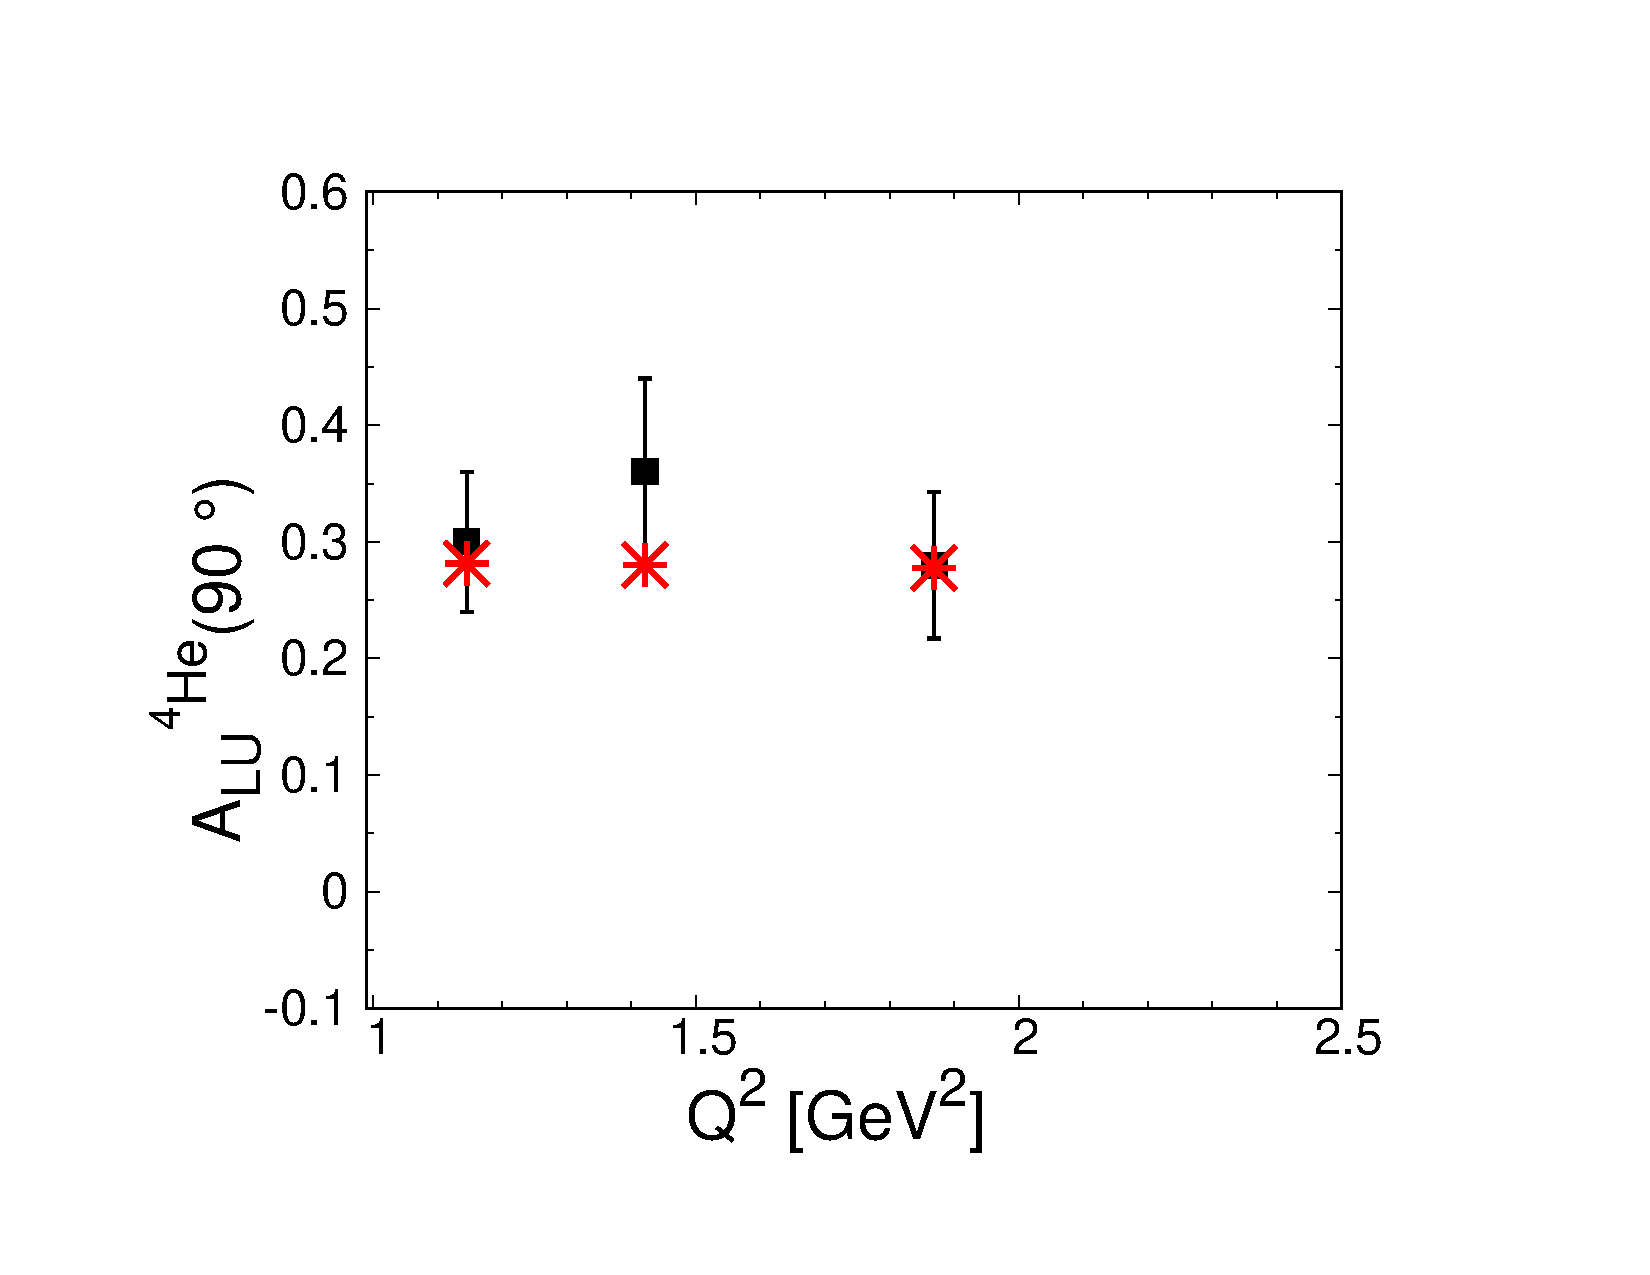
\includegraphics[scale=0.28]{plots/aluq2.pdf}
\vskip -1.cm
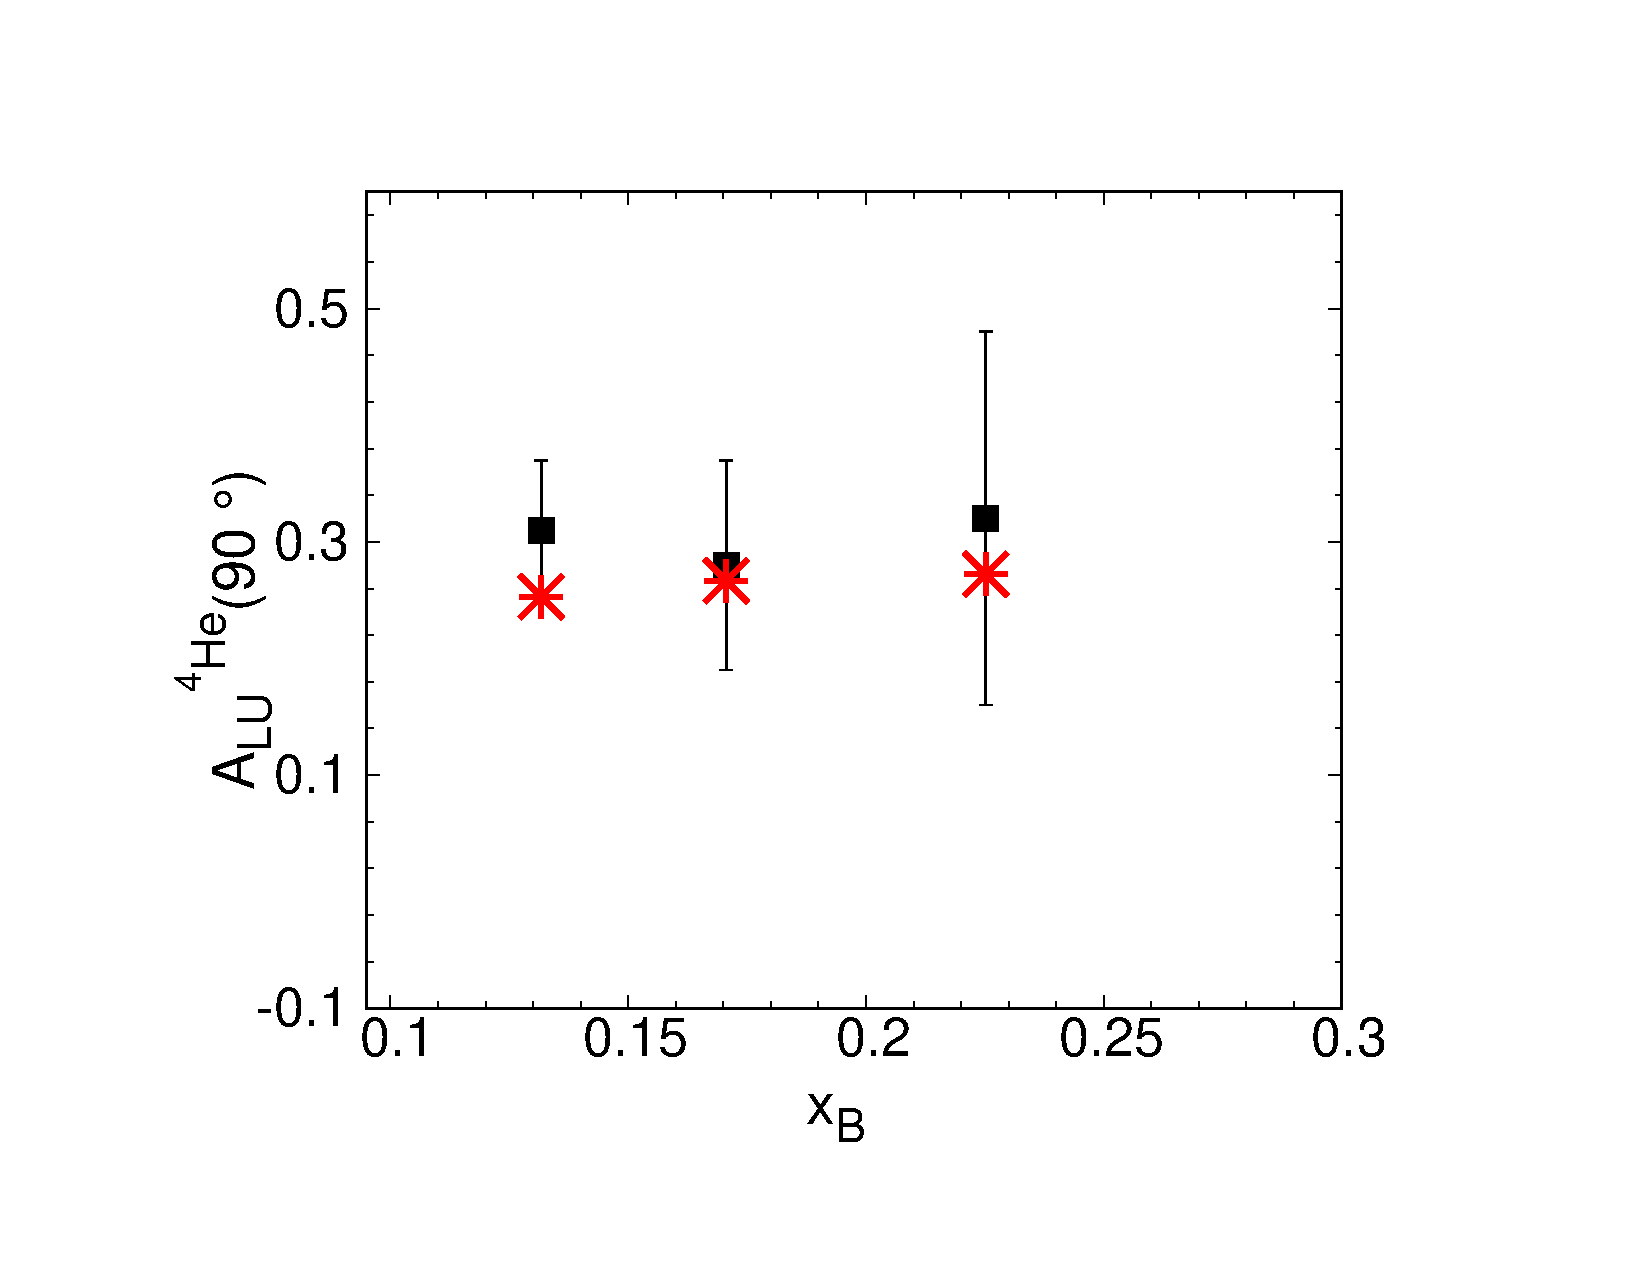
\includegraphics[scale=0.28]{plots/aluxb.pdf}
\vskip -1.cm
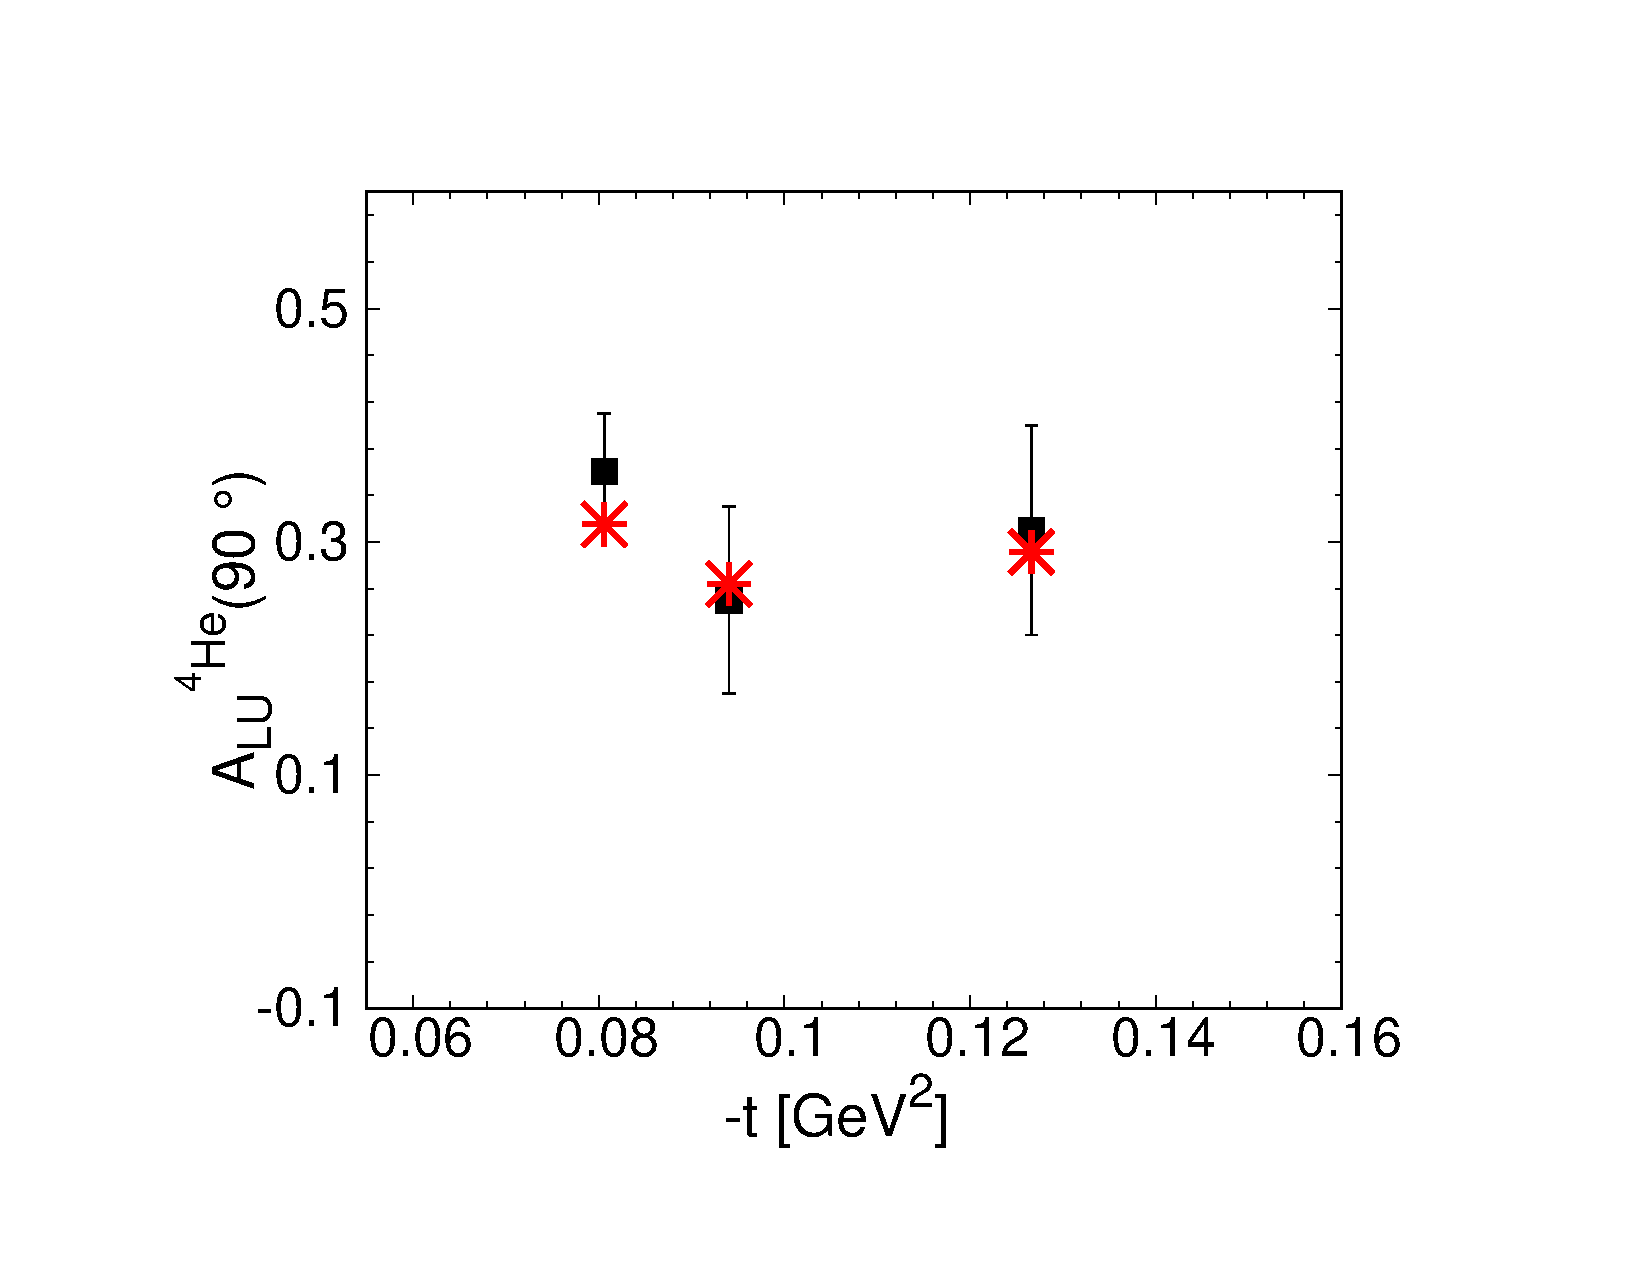
\includegraphics[scale=0.28]{plots/alut.pdf}
\vskip -.5cm
\caption{(Color online) $^4$He azimuthal beam-spin asymmetry $A_{LU}(\phi)$,
for $\phi = 90^o$: results of Ref. \cite{PhysRevC.98.015203} (red stars) compared with data
(black squares)
\cite{Hattawy:2017woc}.
From top to bottom, the quantity is shown in the experimental
$Q^2$, $x_B$ and $t$ bins, respectively. 
}
\label{alu}
\end{figure}

The valence region at intermediate $Q^2$, investigated by 
JLab at 12 GeV, is crucial to access
the most discussed region of the EMC effect.
For light nuclei, such as $^2$H, $^3$He, $^4$He,
a realistic evaluation of conventional nuclear effects,
although sometimes challenging, is possible.
This would allow one to distinguish them
from exotic effects, which could be responsible for
the observed EMC behavior.
Without realistic benchmark calculations,  
interpreting experimental data cannot be conclusive.

%$^2$H is very interesting, both for its rich spin structure
%and for the the possible extraction of neutron information.
%$^4$He, being scalar and isoscalar, and a deeply bound 
%finite nucleus, is ideal to start with.
%In between these two targets, $^3$He provides an opportunity
%to study the $A$ dependence of nuclear effects, and
%it could give an easy access to neutron polarization properties,
%due to its specific spin structure.
%In addition, being isospin-$1/2$, it allows for the
%flavor dependence of nuclear effects could be studied, 
%in particular if parallel measurements 
%on $^3$H targets were possible \cite{Scopetta:2009sn}.

$^2$H is very interesting, both for its rich spin structure
and for the possibility of extracting free neutron information.
As a spin-one object, the deuteron admits a large number of GPDs,
as well as electromagnetic and gravitational form factors (GFFs),
which encode more information than is available in the proton or neutron alone.
For instance, the deuteron appears to have two $D$-terms which encode
the distribution of shear and pressure, while the nucleon has one.
Understanding how forces are distributed in the deuteron
will give significant new insight into the role that QCD plays
in the nucleon-nucleon interaction. DVCS and DVMP on polarized deuterons
will allow much of this rich structure to be extracted.

$^4$He is the ideal deeply-bound nucleus to start with,
since it is scalar and isoscalar, and thus admits a simple
description in terms of its spin and flavor structure.
In between this and $^2$H, $^3$He provides an opportunity
to study the $A$ dependence of nuclear effects, and
it could give easy access to neutron polarization properties,
due to its specific spin structure.
In addition, being isospin-$1/2$, it allows for the
flavor dependence of nuclear effects could be studied, 
in particular if parallel measurements 
on $^3$H targets were possible \cite{Scopetta:2009sn}.

Due to very small cross sections,
especially in the coherent channel where the nucleus does not break-up,
the addressed measurements are very difficult.
Despite this, the first data for coherent DVCS off $^4$He,
collected at JLab, with the 6 GeV electron beam,
have been published \cite{Hattawy:2017woc}.
A new impressive program is on the way at JLab,
carried on by the ALERT collaboration 
\cite{Armstrong:2017wfw,Armstrong:2017zcm,Armstrong:2017zqr}.
Measurements for $^3$He and $^3$H
are not planned, but could be considered
for the upgrade of the ALERT project, at least in the unpolarized 
sector. Polarized measurements, which could
access neutron angular momentum information \cite{Rinaldi:2012pj,
Rinaldi:2012ft,Rinaldi:2014bba}, seem
very unlikely at JLab, due to the difficulty of arranging
a polarized target and a recoil detector very close to each other. 

From the theoretical point of view, a realistic calculation 
of conventional effects for
nuclear few-body systems corresponds to a plane wave impulse approximation 
(IA) analysis. This requires the evaluation of realistic non-diagonal spectral
functions for $^3$He and $^4$He.
For the first target, a complete analysis using the Argonne 18 (Av18)
nucleon-nucleon (NN) potential is available
\cite{Scopetta:2004kj,Scopetta:2009sn,Rinaldi:2012pj,
Rinaldi:2012ft,Rinaldi:2014bba}.
Nuclear GPDs are found to be sensitive to details of 
the used NN interaction.
A study with nuclear ingredients of the same quality
for $^4$He is still missing and should be performed, to update 
existing calculations \cite{Guzey:2003jh,Liuti:2005gi}. 
The evaluation of a realistic spectral functions of $^4$He,
using state-of-the-art NN potentials,
will require the wave function of a three-body scattering state, 
which is a really challenging problem.
Besides, in the incoherent channel of DVCS off $^2$H, $^3$He, $^4$He,
even the study of specific final state interactions will be necessary.

An encouraging approximated calculation has been recently
performed for coherent DVCS off $^4$He \cite{PhysRevC.98.015203}, with the aim to
describe the CLAS data, as an intermediate
step towards a realistic evaluation.
A model of the nuclear non-diagonal spectral function, 
based on the momentum distribution
corresponding to the Av18 NN interaction
\cite{PhysRevC.67.034003}, has been used in the 
actual IA
calculation. Typical results
are found, in the proper limits, for the nuclear form factor
and for nuclear parton distributions.
Nuclear GPDs and the
Compton form factor are evaluated using, as nucleonic ingredient,
a well known GPD model \cite{Goloskokov:2011rd}. 
As it can be seen in Fig.~\ref{alu}, a very good agreement 
is found with the data.  
One can conclude that 
a careful analysis of the reaction mechanism in terms of
basic conventional ingredients is successful and that
the present experimental accuracy does not require
the use of exotic arguments, such as dynamical off-shellness.
More refined nuclear calculations will be certainly necessary for 
the expected improved accuracy of the next generation of experiments 
at JLab, with the 12 GeV electron beam and high luminosity. 

Realistic calculations of $^2$H GPDs and Compton form factors using
state-of-the-art NN potentials are also available~\cite{Cano:2003ju}.
Due to the breaking of Lorentz covariance through a Fock space truncation,
the extraction of gravitational form factors---including those describing
the distributions of mass, spin, pressure, and shear---is ambiguous.
It is possible to model $^2$H GPDs using
a simpler contact interaction while maintaining covariance, and thus
make unambiguous predictions for GFFs and the stress-energy tensor.
This has the shortcoming of using a less realistic interaction,
and is limited to a domain where $t$ is very small. Manifestly covariant
calculations of nuclear structure with more realistic NN interactions
are sorely needed for GPD calculations, since GPDs are the only experimental
avenue through which GFFs can be accessed.
  
While JLab will provide important information
in the valence region, the extension to lower
$x$ values will be possible only at the EIC \cite{Accardi:2012qut}. 
Great opportunities at the EIC are also those related to the possibility
of easily using $^3$H beams, or polarized trinucleon beams and 
recoil detectors at the same time, to access, for example, 
the neutron polarized structure and the flavor dependence 
of nuclear effects.






\section{Short-Range Correlations}
\footnote{Raphael: I merged all the SRC stuff in one sections.}

\subsection{Inclusive Measurements}
Inclusive experiments aim to measure precision cross section ratios at $x >$ 1, a region forbidden to the free nucleon.   Electron scattering probes high-momentum nucleons, typically defined as ones with momenta $\ge$300~MeV/c, a few tens of~MeV greater than the Fermi momentum for a given nucleus (there is a range of values, but for $A>12$, most are around 250~MeV/c). If the presence of these high-momentum nuclei is the result of SRCs, then cross sections for A$>$2 will be re-scaled versions of the deuteron cross sections, signaling more SRCs and therefore more high-momentum nucleons in larger nuclei.   A plateau at $x>$1 in the $A/D$ cross-section ratios would support this picture.    Experimentally, in order to obtain enough data points in $x$ to conclusively observe a plateau, there is a threshold Q$^2$ value.  The onset of the scaling plateau moves to lower $x$ values as Q$^2$ increased, but the threshold has typically been taken to be 1.4~GeV$^2$, illustrated with data from Ref.~\cite{Egiyan:2003vg}.

Cross section plateaus at $x>$1 were observed in several JLab experiments~\cite{Egiyan:2003vg, Fomin:2011ng}.  The ratio is proportional to the relative number of high-momentum nucleons in $A$ with respect $D$.  This is not exactly the same as the number of SRC pairs.   The pairs in a $A>2$ nucleus will experience center-of-mass motion due to the field of the other nucleons.  This will redistribute some strength from the quasielastic peak to the tail of the momentum distribution, resulting in an enhancement in $A>2$ cross sections in the region of interest.  The convention uses $a_2=\sigma_A/\sigma_D$ for raw cross section ratios and $R_{2N}$ for those corrected for the center-of-mass motion of the 2N pair. 


The precision results from JLab E02-019~\cite{Fomin:2011ng} were used to study the nuclear dependence of SRCs. No simple dependence with $A$, density, separation energy or numerous other quantities~\cite{PhysRevC.86.065204} was observed.  However, a deviation of $^9$Be from a simple density dependence analogous to that of the EMC effect was noted.  This led to a number of correlation studies between the two different phenomena and a search for a potential causal effect~\cite{PhysRevC.86.065204, Hen:2012fm, Weinstein:2010rt}.  This is further discussed in Sec.~\ref{sec:SRC_EMC}.

The expectation is to see a second plateau higher in x, in $A/^3\mathrm{He}$ cross section ratios, corresponding to a relative number of 3N configurations in $A$ relative to $^3$He.  Several experiments ~\cite{PhysRevLett.96.082501, Fomin:2011ng, PhysRevC.97.065204}  measured cross sections in the $x>$2 region, but none observed a plateau.  These measurements were done for a range of Q$^2$ values, in order to potentially map out the onset of a 3N plateau, analogously to the case of 2N SRC.  However, defining a kinematic threshold for 3N dominance is more difficult, as there is more than a single configuration that the 3N correlation can take and there are additional dynamics to take into account.  One can consider a simple case of a 3N correlation (1-2) where the momentum of one is balanced by two nucleons (rather than a star configuration).  Solving this problem in $\alpha$, which is a light cone analog for $x$, suggests that to see a second plateau over a meaningful $x$ (or $\alpha$) range requires data at higher Q$^2$ values than any of the experiments have previously obtained~\cite{Fomin:2017ydn}.  Collecting adequate statistics for such a result on $^3$He is time prohibitive, and future experiments will more than likely look for the 3N plateau in $A/^4\mathrm{He}$ ratios.  Just as the 2N plateau is seen more cleanly in $A/^3\mathrm{He}$ cross section ratios, a 3N plateau (if it exists) will reveal itself in  $A/^4\mathrm{He}$ ratios, and more cleanly.  There are several reasons that contribute to this, and they include the fact that the cross section in the denominator is going to zero as we approach $x$ of 2 or 3 (for $A/D$ and $A/^3\mathrm{He}$ ratios, respectively) as well as distortion from center-of-mass motion which does not exist in the nucleus in the denominator. 

\subsection{Exclusive Measurements}
A program of exclusive measurements also yielded interesting results. A series of experiments to measure 2N knockout in a kinematic region of large $P_\mathrm{miss}$ that would correspond to a 2N SRC pair revealed that these pairs are predominantly $NP$~\cite{Subedi:2008zz, Shneor:2007tu}.  This observation was consistent with the theoretical calculation~\cite{Schiavilla:2006xx} showing a tensor force dominance in the regime where the first measurements were done and also predicted a weakening of $NP$ dominance with growing $P_\mathrm{miss}$, which follow-up measurements appear to support~\cite{Korover:2014dma}, although with uncertainties that prevent conclusive statements. 


%\subsection{SRC Summary}
%Going into the 12~GeV era at JLab, our future measurements are informed by the following lessons from previous experiments
%\begin{itemize}
%\item Scaling of $A/D$ cross section ratios at $x>$1 observed
%\item No clear nuclear dependence of the $a_2$ ratios
%\item $NP$ dominance of SRC pairs (while significant contributions from FSI are present, they are unlikely to mimic the physics result)
%\item No 3N SRC plateau observed
%\end{itemize}
\subsection{\label{sec:SRC_EMC}SRC- EMC connection}
While neither SRCs or EMC effect showed a simple nuclear dependence, both exhibited the same nuclear outliers. Several analyses were done to examine the correlation between the two physical phenomena~\cite{PhysRevC.86.065204, Hen:2012fm, Weinstein:2010rt}.  On the surface, it might very well be a coincidence: SRCs are a measure of quasielastic cross sections, whereas the EMC effect probes DIS quark distributions.  Yet, there is room for the two to be related, as the cause for the nuclear modification of structure functions is not understood, and it could come from short-range dynamics probed by SRC measurements.   The other possibility is that both effects arise as the result of the same underlying mechanism rather than having a causal relationship.  Multiple corrections to SRC and EMC measurements were applied to check the robustness of the correlation, but the existing measurements are not precise enough nor span enough nuclei for any meaningful conclusions to be drawn.  Recent work in % FIXME Ref~\cite{} 
proposes a new model for this that consists of a free structure function piece as well as a piece that depends on SRC. Because of the np dominance of SRC, this reduces the EMC effect to a universal modification with an amplitude mostly depending on the number of protons in the nucleus.  \footnote{Raphael: That was a significant short cut, hopefully this phrasing is a bit more clear.}
\begin{figure}[htb]
  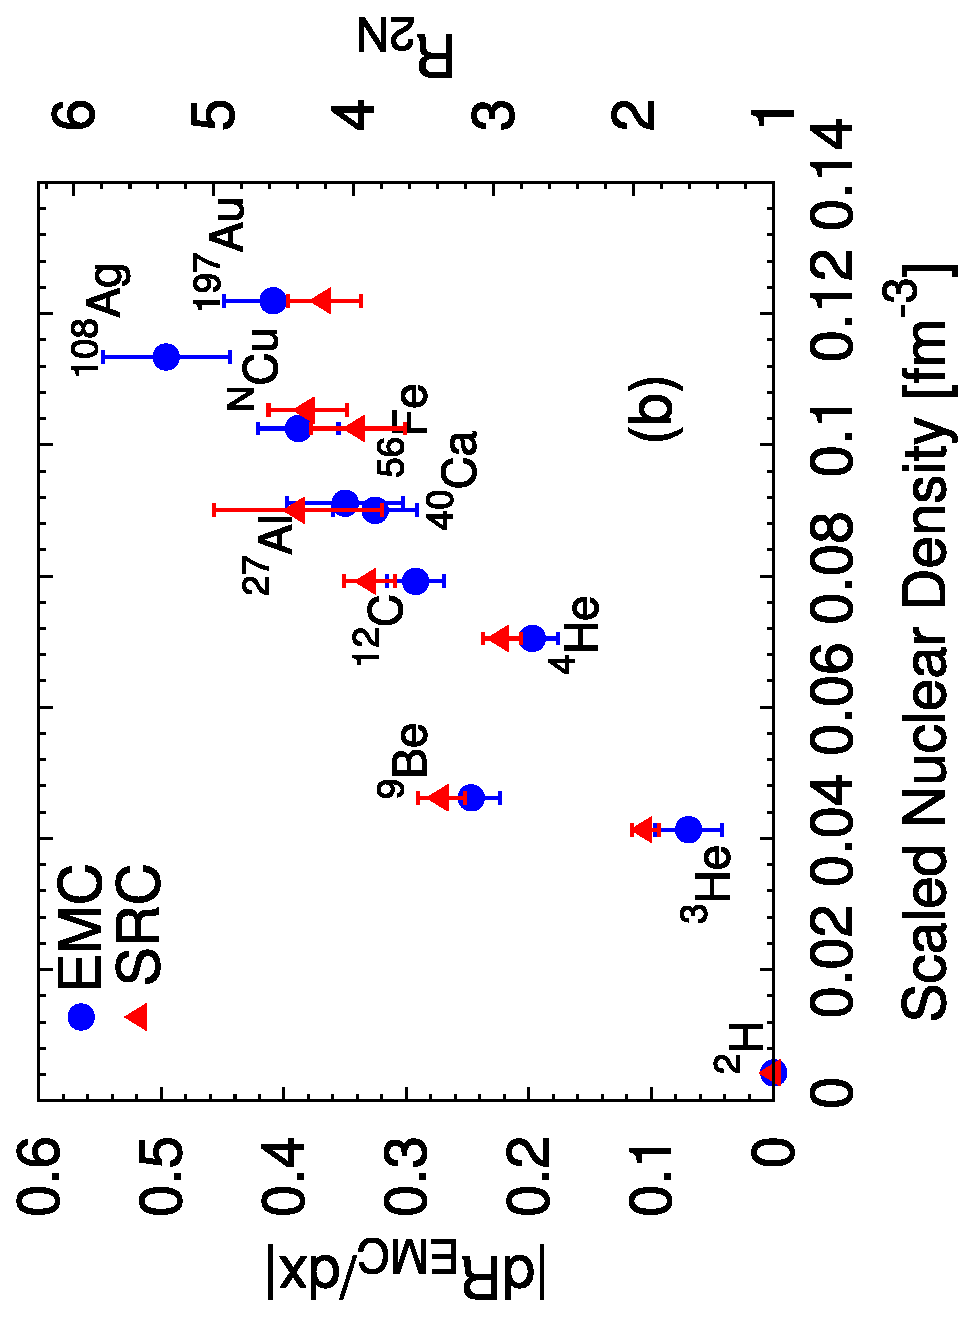
\includegraphics[angle=270, width=0.45\textwidth]{plots/emc_src_vs_scaled_dens_all.eps}
  \caption{Size of the EMC effect (left axes) as well as the number of SRC pairs (right axes) as a function of scaled nuclear density}
  \label{fig:src_emc}
\end{figure}

\subsection{Quarks at $x>$1}
Quasielastic kinematics at $x>$1 probe moving nucleons, but if we increase the Q$^2$, the inelastic contribution begins to dominate, allowing us to access quark distributions. Existing JLab data have a limited range in $x$ and require the application of the of so-called "target-mass corrections" (TMCs) to extract the Q$^2\rightarrow\infty$ structure function limit.  This analysis was done for the E02-019 data, showing that the data are on the edge of... being useful?



\section{Probing the nucleus with tagged reactions} 

Medium modification is not limited only to differences in the PDFs,
but could also be manifest in other observables, such as the elastic nucleon form factors.
This idea
triggered several experiments to measure the quasi-elastic 
process ($e+A \rightarrow e+p+X$). In this process, the 
elastic scattering occurs on a bound nucleon and allows the extraction of its modified 
form factor. One of the expectations from these measurements was to detect a change
in size of the bound nucleon compared to the free one. This has also motivated 
DVCS experiments, where a similar process is accessible, the so-called
incoherent nuclear DVCS ($e+A \rightarrow e+p+\gamma+X$). Results for these two 
channels are presented in Fig.~\ref{fig:QEincoh}, and show in both cases a 
significant deviation between the bound and the free nucleons. 
The difficulty with the interpretation of these measurements lies into the 
effect of final-state interactions. Indeed, the reaction products are likely
to re-interact with the remnants of the nucleus, and this affects significantly the
results. The calculation of these final state effect is complex and leads to large model 
uncertainties. 
Another problem is that in the calculation of these processes, it is important
that the initial and final-state nucleons are the same. This cannot be guaranteed
in a nucleus where one can have a off-shell nucleon in the initial state or 
have processes where a charge is exchanged and a neutron becomes a proton. For
these reasons, the debate remains open around 
the interpretation of the data on bound nucleon scatterings~\cite{Benhar:2006wy}.

\begin{figure}[tbp!]
\center
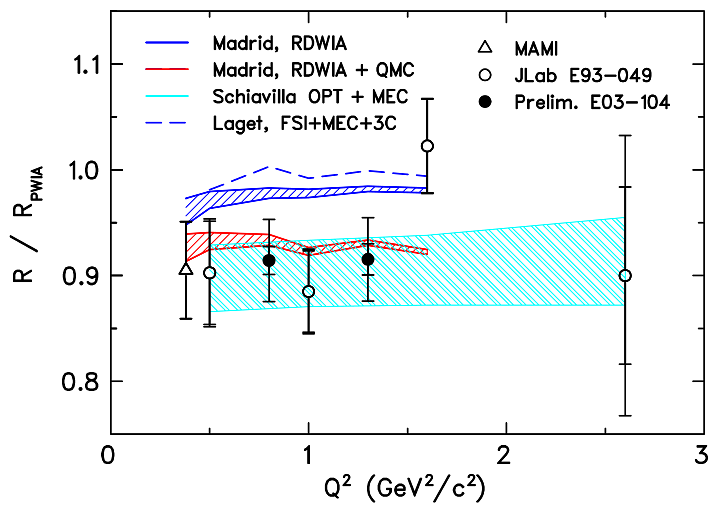
\includegraphics[width=7.6cm]{plots/ModifiedFF.png}
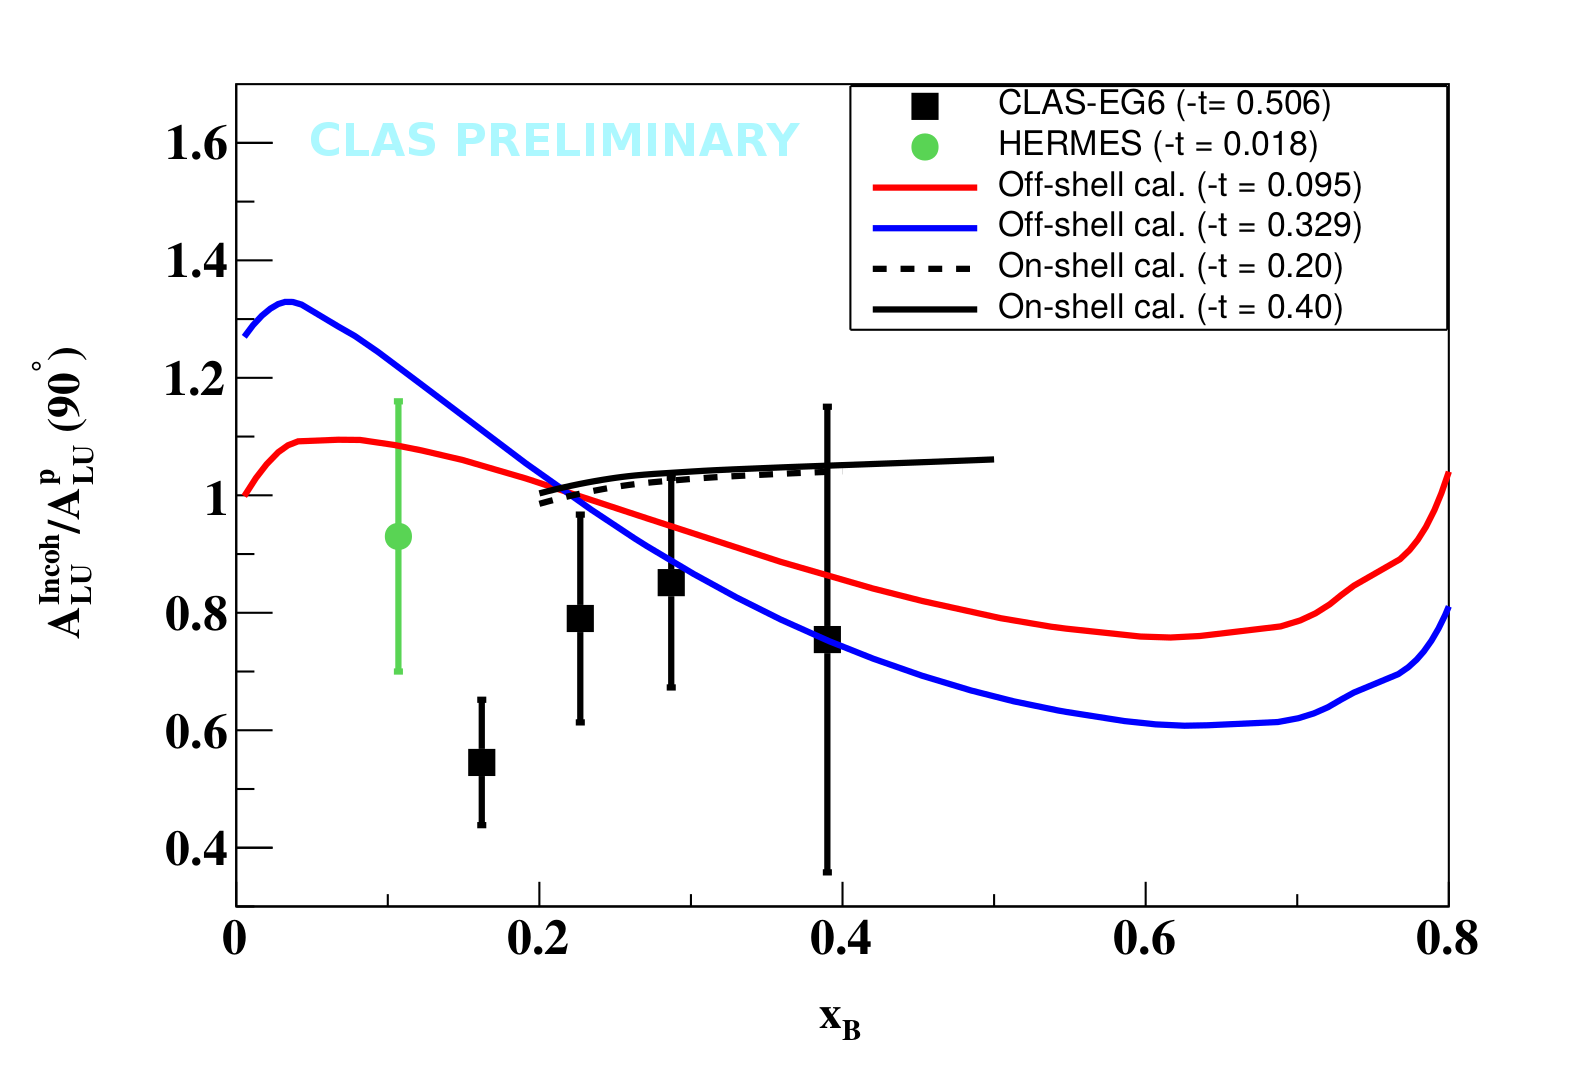
\includegraphics[width=8.5cm]{plots/ALU_ratioInc_x_shortscenrario.png}
\caption{Left: results of \cite{Strauch:2002wu} for the quasi-elastic form factor relative to
the plane wave impulse approximation. Right: CLAS preliminary results 
for the beam spin asymmetry in incoherent nuclear DVCS relative to the free proton DVCS.}
\label{fig:QEincoh}
\end{figure}

The solution to these problems is the tagging method, in which the nuclear fragments
are detected as illustrated in Fig.~\ref{fig:size} for the simplest case, deuterium.
In this process ($e+d \rightarrow e+p_s+X$), the high-energy electron is measured
together with the low-energy proton. The measurement of the proton in the backward 
direction ensures that it was not part of the hard interaction, thus noted with 
the $s$ subscript for spectator, and transforms the deuterium into 
an effective neutron target. First results of such a measurement
have been reported in~\cite{Baillie:2011za} with the goal to extract the structure
function of the neutron. We show in Fig.~\ref{fig:wstar} a result of this experiment
comparing the invariant mass obtained with and without the tagging method. It is 
clear that the tagging method gives a much better resolution of the structure 
present in the invariant mass distribution. Similarly to the measurement presented in 
the previous section, the main result of this experiment was however limited by the lack
of statistics. Yet, this successful measurement of a tagged process opens the way for more
experiments of the same kind in the future. 

\begin{figure}[htbp!]
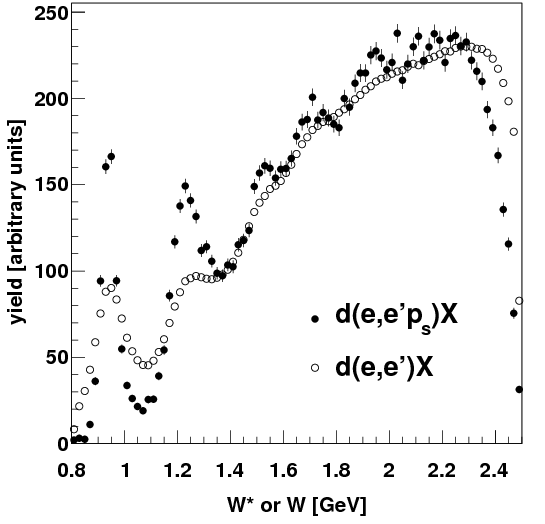
\includegraphics[width=6.1cm]{plots/Wstar.png}
\caption{Neutron-electron invariant mass obtained from tagging (full points) compared 
to the invariant mass obtained
from deuterium data (hollow points)~\cite{Baillie:2011za}.}
\label{fig:wstar}
\end{figure}

The nuclear remnant tagging is the extension of the deuterium tagging to heavier nuclei, which
consists in measuring the reaction ($e+A \rightarrow e+(A-1)_s+X$), with
$(A-1)_s$ the spectator remnant of the nuclear target. This measurement is very 
interesting as it gives a direct information on which nucleon was hit by the 
deeply inelastic electron scattering in the nucleus. Also, by selecting 
low momentum backward emission of the $(A-1)_s$, we can suppress the 
final state interactions that are often a problem in such nuclear reactions. 
Detailed studies~\cite{CiofidegliAtti:2003pb,Alvioli:2006jd} have indeed shown 
that the final state interactions effects are minimized when the nuclear recoil
is detected in a backward angle relative to 
the virtual photon direction and maximized in perpendicular kinematics.
The detection of such recoil nuclei is however extremely challenging.

Tagging recoiling remnants has another interest in the quest to understand nuclear structure.
The kinematics of the nuclear remnants contain information on the
initial state of the nucleons in the nucleus. By performing at the same time the 
tagging and a deeply inelastic scattering, we probe simultaneously the nucleon and the 
quark structure of the nucleus. Tagging is therefore a unique tool to relate the EMC
effect to more classical nuclear effects and observe if there is any correlation between
them. The more natural variable to use for these studies is the nucleon virtuality.
It can be calculated~\cite{CiofidegliAtti:2007ork} in the impulse 
approximation, where the nucleon momentum is exactly $\mathbf{p} = -\mathbf{P}_{A-1}$, 
giving
\begin{eqnarray}
    v(|\mathbf{p}|, E) &  =  & \left (M_A - \sqrt{(M_A - m_N + E)^2 + \mathbf{p}^2} \right )^2  \\* \nonumber
                    & & -  \mathbf{p}^2 - m_N^2,
\end{eqnarray} 
where $E$ is the removal energy, $M_A$ the mass of the target nucleus
and $m_N$ the mass of the nucleon. The nucleon virtuality is a key 
observable to understand the nuclear quark and gluon structure,
as there are radically different predictions for its impact on the partonic structure.
Indeed, the descriptions of the EMC effect based on nucleon dynamic 
predict a strong correlation between virtuality and nucleon modification,
while the ones involving other hadronic degrees of 
freedom or mean field effects do not. 

Nuclear tagging measurements have never been performed in the past
on nuclei with $A>2$ due to detector limitations. Indeed, the radial TPC used 
for the experiments described above~\cite{Baillie:2011za}
is unable to differentiate isotopes and thus ensure the identification of 
nuclear remnants. There are plans at JLab to remediate this issue
with the construction of a new detector to perform nuclear tagging measurements 
for the first time~\cite{Armstrong:2017zqr,Armstrong:2017zcm}.


\section{Systematics}
\subsection{Nuclear Dependence of $R=\sigma_L/\sigma_T$}


Due to the relatively low energy of the 6~GeV JLab E03-103 measurements, effects due to acceleration and
deceleration of electrons in the Coulomb field of the heavier targets (Cu and Au) could not be ignored.
However, once applied, these so-called Coulomb corrections resulted in ratios systematically larger
than those found by previous experiments.  This apparent discrepancy motivated the re-examination of
earlier measurements, and it was found that, while the bulk of the large $x$ measurements from SLAC
were taken at significantly higher beam energies, SLAC E140 (an experiment dedicated to studying
the nuclear dependence of $R=\sigma_L/\sigma_T$) had used beam energies similar to JLab E03-103, but for
those measurements had not applied Coulomb corrections.  Once Coulomb corrections were applied to the E140
results, the conclusion that there was no evidence for a nuclear dependence of $R$ was less strong, with
$\Delta R=R_A-R_D$ about 1.5 standard deviations from zero. Further, when a combined analysis
of available SLAC E139, E140, and JLab E03-103 data was performed for data at $x=0.5$ and $Q^2\approx5$~GeV$^2$,
a similar deviation of $\Delta R$ was found~\cite{Solvignon:2009it}.

This result, combined with hints of a difference in $R$ for protons and deuterium motivated a 
new experiment to make further measurements of the nuclear dependence of $R=\sigma_L/\sigma_T$
with better precision than E140 and for a wider range of $x$ and $Q^2$ than previously
measured~\cite{12gev_nucr}.  This experiment will provide precise measurements of $R=\sigma_L/\sigma_T$
for the nucleon for $0.1<x<0.6$ and $1<Q^2<5~\text{GeV}^2$ as well as determination of $\Delta R= R_A-R_d$ for the same
kinematics using a copper target. Additional data will also be taken with carbon and gold targets for a subset
of the kinematics.


\subsection{Hadronization and Final State Effects}

The formation of hadrons and the propagation of quarks in a nuclear medium is important for interpeting the final states of reactions in SIDIS and Drell-Yan processes as well as critical in interpreting gluon distributions.  An important open question are the relative sizes of the interactions between asymptotic quark propagation and interactions after hadronizatoin.  As final states can reveal important information regarding the kinematics (such as Bjorken $x$) and flavor in a given interaction, improving the quality studies and models will simultaneously improve the extraction of modification data.  Studies have taken place at a variety of facilities, e.g. Fermilab~\cite{PhysRevC.75.035206}, JLab~\cite{PhysRevLett.99.242502, ELFASSI2012326}, and HERMES~\cite{Airapetian2011} as well as a future program with CLAS12 at JLab to study this in a broad set of channels~\cite{quarkformprop}.

Determination of the gluon distributions are also contaminated by final state interactions. nPDFs have been including routinely particle production in $d+\mathrm{Au}$ collisions into the fits, an observable that is very sensitive to both the initial state and hadronization of the gluon. The fragmentation functions for pion production have been best determined from $e^+e^-$ data, though the fragmentation of gluons have a sizable theoretical uncertainty. Data from the LHC at $7$~GeV can not be well described by a global fit unless a significant cut in $p_{T}$ is applied to the data, leaving out a relevant portion of the covered $d+\mathrm{Au}$ region.  With the present data, this constitutes a sizable source of uncertainty for the extraction of the nPDFs and conclusions from incorporating particle production data from hadron colliders into the fits must be drawn carefully.

\subsection{Free Nucleon Parton Distributions}

While the free proton parton distributions have been studied extensively and with great precision, there still remain important measurements to be done to constrain the two leading-flavor parton distributions, in particular in the ratio of $d/u$ limit as $x \rightarrow 1$.  As these represent the basis of comparison for any nuclear modification effect, it is critical to have high quality data available, especially as one considers doing flavor decompositions of nuclei.  There are several programs which intend to improve the fixed-target lepton scattering data, such as using the ratio of ${}^{3}$H and ${}^{3}$He cross section~\cite{mar}, tagged spectator with deuterium~\cite{bonus12}, and parity-violating deep inelastic scattering on the proton~\cite{solid_pvdis}.  In addition, recent analyses of $W$ and $Z$ production in $p\bar{p}$ collisions from the CDF and D\O\ collaborations~\cite{D0:2014kma,Abazov:2013dsa,Acosta:2005ud,Aaltonen:2009ta,Aaltonen:2010zza,Abazov:2007jy} have also provided new constraints at large $x$ and have been incorporated into a recent global PDF analysis~\cite{Accardi:2016qay}.


\section{Summary - Recommendations}

The challenge for the next era of understanding medium modification is clear and the path to answer to key questions is open. 
\begin{itemize}
\item What is the isovector nature of the EMC effect?  This requires a set of high-precision experiments across nuclei of traditional inclusive cross section ratios, electroweak measurements which are sensitive to unique quark flavor combinations, and Drell-Yan experiments.  These would be complemented by exclusive isotope tagging experiments. 
\item What is the spin dependence of the EMC effect?  There is no experimental information available and any such measurement would break into new ground and would provide new information on potential mechanisms.
\item What is the transverse momentum depedence of the EMC effect?  This can be addressed through tagged scattering measurements which can separate local density and mean field mechanisms.   

\item What is the Full Nucleus Image (in terms of quarks and gluons), deuteron specifically, potential EIC details
\end{itemize}

We are grateful to the ECT* for hosting the workshop which made this work possible.


\bibliography{fullbib}

\end{document}



